\documentclass[11pt]{article}
\usepackage[top=1.00in, bottom=1.0in, left=1.1in, right=1.1in]{geometry}
\renewcommand{\baselinestretch}{1}
\usepackage{graphicx}
\usepackage{natbib}
\bibliographystyle{agsm}
\usepackage{amsmath}
\usepackage{xcolor}
\usepackage{lineno}
\usepackage{xr-hyper}
\newcommand{\R}[1]{\label{}\linelabel{#1}}
\usepackage{todonotes}

\def\labelitemi{--}

\begin{document}
\renewcommand{\refname}{\CHead{}}

\title{Effects of phenology on plant community assembly and structure }
\author{Elsa E. Cleland* \& E. M. Wolkovich*}
\date{\today}
\maketitle


\setlength{\parindent}{0cm}
\setlength{\parskip}{5pt}
*Authors contributed equally.

\begin{abstract} % 150 words max
Phenology---the timing of critical stages of growth and reproduction and the transitions between them---determines environmental conditions and biotic interactions. Hence, phenology is a key functional trait influencing organisms' survival and fitness; however, the role of phenology in community assembly processes has been less considered. Here we review the importance of phenology in environmental and biotic filtering, structuring priority effects, and species coexistence, in the context of the assembly of native communities, as well as in invasions and restoration. We highlight the complexity of the life history aspect of phenology, which makes simple trade-offs---such as between growth timing and competitive ability---part of larger plant strategies shaped by a framework of risk, reward and investment over multiple timescales. Embracing this complexity could yield insights into how phenology shapes communities.
\end{abstract}

\emph{Keywords}: life history events, germination, leafout, plant traits, seasonal priority effects, constraints

\section{Main text}
\linenumbers
\subsection*{Introduction} 

Phenology, defined here as the timing of growth and reproduction, is a key plant trait because it is often closely tied to the fitness of individuals in seasonal environments \citep{verdu2005early,munguia2011meta}. Phenology determines both the environmental conditions and biotic interactions experienced by individuals during different stages of their life-cycles \citep{donohue2005niche}, and hence the relative impact of these factors on survival and reproduction \citep{caruso2019meta}. For instance, in temperate ecosystems, the timing of leaf emergence or flowering in spring can determine fitness consequences of frost events \citep{inouye2008effects,augspurger2013reconstructing}, or the impacts of herbivores \citep{meineke2021phenological}, on plant performance.

Plant phenology has also garnered global attention because observations suggest that phenology of many plant species has shifted in recent decades, associated with rising temperatures and co-occurring global changes \citep{wolkovich2012warming,parmesan2015plants,menzel2020climate}. In response to both experimental and observed warming, plants generally display earlier spring events (e.g. leaf-out, flowering) and later fall events \citep[e.g. senescence,][]{Henry:1997lg,menzel2020climate}. However, there is considerable variation among species in how much they shift their phenology \citep[][sometimes termed `phenological sensitivity']{cook2012divergent,wolkovich2012warming,konig2018advances}. Species that `track' climate change by accelerating early-season phenology appear to maintain or even increase their performance in experimental settings \citep{cleland2012phenological,wolkovich2021phenological}. Hence, species-level phenological responses to global changes have the potential to influence processes at population- \citep{iler2021demographic}, community- \citep{cook2012divergent,caradonna2014shifts}, and ecosystem-scales \citep{piao2019plant}.

Phenology is one of many interacting functional traits that influence the suitability of an organism to its environment. Functional traits---defined as morphological, physiological or phenological traits that``impact fitness indirectly via their effects on growth, reproduction and survival" \citep{violle2007let}---are at the core of many theories in community ecology, especially those aiming to predict the assembly of local communities from a larger regional species pool. Despite the recognized importance of phenology for understanding species responses to the environment, and structuring species interactions in communities, phenology is missing from many frameworks seeking to identify major axes of global plant trait variation \citep[e.g.][]{westoby1998leaf,wright2004worldwide,diaz2016global,joswig2022climatic}. Yet, many recognize that phenology is essential in trait-based approaches to understanding species interactions and community assembly \citep{cope2022role}.

Here we focus our review on the role that phenology plays in plant community assembly. We examine how phenology enters into major theories of community assembly, including the potential for phenology to influence competitive and facilitative interactions, and to shape priority effects and coexistence. Including phenology in such theories highlights a suite of ecological and life history trade-offs that may occur with different phenological events over different timespans, and in the many different environmental contexts humans have created today. We thus include in our review studies that document community assembly following disturbance, shifting community composition in response to global environmental changes, and the role that phenology plays in invasion by exotic species into resident communities, including efforts to assemble native communities that are resistant to invasion through restoration. 

Given our focus on community assembly, we consider mainly multi-species studies from ecological perspectives. We therefore do not consider purely ecosystem-level measures of phenology, the underlying environmental cues and cue systems for plant phenology \citep[for a review see][]{chuine2017process}, nor---relatedly---how multiple global change factors interact to influence phenology \citep[e.g.][]{zhou2023climate}. Although evolutionary processes can influence community assembly \citep{cavender2019diversification}, a review of evolutionary responses of phenology to global changes is beyond the scope of this review. However, we take an evolutionary perspective to show how selection may act on phenology in ways that shape assembly and trait trade-offs.

\subsection*{Defining phenology} 

We define phenology as the timing of critical stages of growth and reproduction and the transitions between them. \R{defineS}This definition is intentionally more inclusive than some other definitions, which focus on recurring or seasonal events, and thus can narrow phenology to only certain plant types or biomes (e.g., woody species in the temperate zone). We find this narrowing artificial and think it can limit a broader understanding the selective pressures on phenology that---as we outline below---are critical for understanding the role of phenology in community assembly. Our definition thus includes both leafout of trees and seed germination of annual plants, at the same time that it encompasses fruiting, flowering and transitions in and out of these phases, such as dormancy and vernalization (Fig. \ref{fig:phenologycircles}).\R{defineE}

Our definition, like many, still obscures much of the underlying complexity of most phenological `events,' such as leafout or fruiting. First, while `event' suggests an almost instantaneous timepoint, this is a gross simplification. Phenology is an attempt to extract and simplify the temporal dimensions of various developmental processes that can rarely (if ever) be one point in time. Instead, phenology is generally a series of distributions. For any one event within one individual, there is a distribution of the process starting, peaking and ending, which can be variously imagined as a normal curve or sigmoid curve (imagine the event of a grape cluster ripening: the number of berries ripening each day mapped over time would be normally distributed, while the progress towards all berries ripened would be sigmoid). This then scales up across individuals within a population, and across populations \citep{inouye2019}. Such complexity is generally simplified into an `event' that often represents the 50\% point extracted statistically after repeated observations over time. 

Second, phenology---as a point in time---can appear highly flexible or strongly fixed---depending on how time is defined. To date, much work has used calendar time for phenology: a wildflower flowers on a certain day of the month in one year, for example, and on another day another year. When measured this way, phenology appears highly flexible---jumping around in temporal space from year to year or place to place---as the environment is variously warm, cool, dry or wet. Yet, plant phenology can also appear highly deterministic when defined in biological time; that is, when defined as relative to a set of known environmental triggers, such as accumulated cool temperatures known to vernalize some flowering species. When the underlying triggers or cues for phenological events are fairly well understood for some events (with perhaps flowering in \emph{Arabidopsis thaliana} being the best understood) phenology can be highly predictable and effectively---inflexible. The first definition is relevant for localized studies of community assembly, while the later is preferred for predictive models because it removes some of the spatial and interannual `noise' in the environmental cues that trigger phenology.

\subsection*{Phenological assembly: From the abiotic to biotic environments} 

Communities assemble from a pool of potential species through a series of abiotic and biotic sorting processes \citep{hillerislambers2012rethinking}. At the largest scale, a community's assemblage is limited by species present in a wider regional pool---species well suited to an environment will thus not occur in any one local community unless they are present in this regional pool. From this pool, species are filtered based on the abiotic environmental conditions of a particular location---species must be able to persist through a local environment's extremes in hot, cold, dry, wet and other factors to pass through this `environmental filtering' step of assembly. This collection of potential species that could form a community is also filtered once more---by the now smaller, local pool of species itself \citep{hillerislambers2012rethinking}. 

Competitive, facilitative, predatory and all other biotic interactions determine which species together can co-occur in the long term. If two species compete too strongly, then only the stronger competitor will remain in the local community at this step. Similarly obligate mutualists, predators and parasites will persist only if the other species they require are present in the community. This final stage of assembly is where much of community ecology has focused over its history as a subdiscipline---deriving theories of coexistence, including whether species even truly `coexist' or merely are on a slow walk to extinction for all but one species in each community \citep{Hubbell:2001vo}. 

Phenology enters community assembly at both the environmental (abiotic) and biotic filtering steps. Species phenologies must match the environment to pass the first filter: their growth and reproduction must be timed to match periods when the environment is mild and resource-rich enough for these events \citep{rathcke1985phenological}. Thus, in an environment with cold sub-freezing winters, species generally must have well-timed dormancy to avoid growing too much in the middle of the winter when they would lose new tissue. Similarly, arid and tropical environments impose filters against certain phenologies. Once a set of species passes the environmental filter, phenology matters again at the biotic filtering step, where species with too similar phenologies may compete too strongly to co-occur \citep{gause1932experimental, abrams1983theory}.   Alternatively, species that overlap phenologically have the opportunity to develop facilitative interactions \citep{duchenne2021phenological} promoting co-occurrence, while species with little phenological overlap are unlikely to interact via biotic filtering processes. Interactions with predators (herbivory) may either limit or promote long-term persistence, depending on the dynamics \citep[such dynamics relate in part to a larger literature on trophic synchrony, for which we refer readers to a number of recent reviews, e.g.][]{kharouba2018global}.

The importance of phenology to species passing the environmental filter of community assembly has been long studied---though rarely framed in exactly these terms. Early studies of the controls on species ranges stressed phenology as a major axis \citep{salisbury1926geographical}. Today process-based models based almost entirely on species phenology are highly predictive of tree species ranges \citep[where they have been tested,][]{chuineJTB,Morin:2009gt,morin2007}. These models integrate over both growth and reproduction: trees in temperate systems leafout, flower and fruit then lose tissue to frost if temperatures dip below their cold limits (which vary for leaves, flowers and fruit), they then must have a long enough season for fruit development. Various species along various range edges are limited by tissue damage, fruit ripening or carbon starvation---depending on the summed outcome of a phenological model \citep{Chuine:2010gm}. 

Range models based on phenology highlight the life history challenges of phenology---species must fit in a sequence of events to grow and reproduce within environmentally feasible periods. Through this lens, the sequence and length of phenological events becomes critical, and prevalent trade-offs from life history theory become more relevant. For example, trade-offs between fruit size and time available to grow (growing season length) may drive some species to flower before they leaf \citep{dan2021nph}. Similarly, trade-offs between growth, reproduction and survival may determine how often an individual invests in reproduction \citep{schaffer1974optimal,law1979cost,stearns1998evolution}. These complexities are present in many process-based models, but rarely extend beyond into either life history or community ecology theories. Process-based models similarly view phenology often as a static trait that shapes broad-scale (biogeographical) processes \citep{Chuine:2010gm}, with little focus on the role it may play within communities. Yet plant invasions suggest this view is overly narrow.

Recent work on plant invasions suggest a role for phenology beyond environmental filtering and instead through biotic assembly mechanisms \citep{wolkovich2011phenology,Fridley:2012fj}. Theory in invasion biology focuses both on the characteristics of the species invading, and on the community into which it invades, with the vacant niche model proposing that species should invade if there is open `space' in a community and the invader fits that space \citep{Elton:1958bk}. Phenologically, this predicts species do not pass through a filter simply based on their phenological match to the abiotic environment, but on their match to the biotic environment as well. Invaders should thus take advantage of open temporal space within communities, which some evidence suggests they do---particularly at the start and end of seasons (see next section). 

Findings from invasion biology support a potential role of temporal niches more broadly in community assembly \citep{gotelli1996}. Static environments (e.g., a chemostat) cannot easily support temporal niches, but even slightly more complex dynamics of resource availability across a season can create the potential for temporal niches\R{morefsS} \citep[Fig. \ref{fig:resource}, and see][]{Chesson:2004eo}, \R{notincluded1S}though little work has examined this\R{notincluded1E}. Models including a simple resource pulse that starts a growing season can theoretically create space for temporal niches and thus phenological assembly \citep[discussed further in the section on coexistence, and see][]{wolkovich2021phenological}. Such models, however, highly simplify the resource dynamics of most environments, which is more aptly described a multi-dimensional mosaic of access to light, water, and nutrients variously present through abiotic factors (weather, tree fall due to storms etc.) and lost through uptake and use by other species \citep{craine2013mechanisms}. \R{morefsE}This complexity leaves much room for the order of species arrival to matter.

\subsection*{Priority effects}

In addition to the roles of environmental filtering and biotic interactions for determining the temporal niches of species in assembled communities, the relative timing of arrival of a species can influence community assembly through priority effects \citep{alford1985priority,chase2003community,fukami2015historical}. Priority effects have often been considered as historical contingencies in the process of community assembly, arising from the chance establishment of individuals of different species, resulting in different community compositions across sites that are otherwise similar in terms of species pools, environmental conditions and disturbance histories \citep[e.g.][]{diamond1975assembly}. In the context of succession, early studies noted that the timing of disturbance relative to seasonality of seed dispersal could result in different species initially colonizing sites, and variation in later species abundances \citep{keever1950causes,holt1972effect}. More recently, the seasonal order of species’ growth onset has also been found to influence species' relative abundances in communities, via priority effects \citep{fukami2015historical,wainwright2012seasonal,rudolf2019role}.  Phenology is a key aspect of a species niche, and hence should be key to niche-based predictions of community assembly \citep{vannette2014historical}.

The predictive power of priority effects for understanding community assembly suggests that the potential for competitive exclusion is not equal across the growing season, and should drive patterns where phenologically earlier species are competitively dominant. For instance, the timing of germination is a trait which is highly linked to plant fitness, because it determines both the biotic and abiotic environment experienced by the emerging seedling \citep{donohue2010germination}. Foundational studies demonstrated that earlier germinating individuals achieved higher adult size, likely via space and resource preemption, and competitive suppression of later germinating individuals of the same species \citep{ross1972occupation},  a type of asymmetric competition \citep{connolly1996asymmetric}. Subsequent work has found repeatedly that earlier germinating species gain a competitive advantage over later germinating species \citep{cleland2015priority,waterton2016trade,blackford2020species}. Hence it is unsurprising that seeds can “sense” the presence of neighboring seeds, and display accelerated germination in more competitive environments \citep{dyer2000accelerated}.

However, a number of factors can reduce the benefit of early germination phenology. For instance, apparency to herbivores \citep{waterton2016trade} or exposure to sub-optimal conditions such as early-season drought \citep{wainwright2012seasonal} can create trade-offs whereby later germinating species can achieve numerical dominance. Further, priority effects are not always competitive; experimental work with \textit{A. thaliana} has shown that individuals germinating during stressful periods of the growing season can be facilitated by neighbors \citep{leverett2017germination}. This finding is broadly consistent with the prediction that competitive priority effects will be stronger under conditions of high resource availability or low stress \citep{vannette2014historical}, opening the door for facilitative priority effects to arise under stressful conditions.

Priority effects arising via differential germination timing are likely to be most important in herbaceous-dominated ecosystems, but may also arise in woody-dominated ecosystems via the timing of spring green-up, due to light preemption by species with earlier growth dynamics. For instance, the non-native Amur honeysuckle (\textit{Lonicera maackii}) invades the understory of deciduous forests in the Eastern U.S., where it has earlier leafout in the spring likely associated with greater frost tolerance compared with co-occurring native shrubs \citep{mcewan2009leaf}. The potential for priority effects to arise directly from earlier season flowering are less clear mechanistically, and early-flowering species are more prone to frost damage in temperature ecosystems \citep{inouye2008effects}. However, the timing of flowering can be indicative of the timing of soil resource uptake, with important implications for community assembly \citep{gulmon1983phenology,seabloom2003invasion}.

Climatic context also influences phenological priority effects. Inter-annual climate variation \citep{levine2011seasonal}, or directional changes in climate, can change the relative order of species seasonal phenology or the correspondence of temperature and moisture cues (\cite{kimball2010contemporary}, resulting in altered species interactions and species relative abundances \citep{thomson2017between,kimball2010contemporary,buonaiuto2023contrasting}. Thus, seasonal priority effects will likely play a key role in understanding changing species compositions in plant communities with future climate change.

Restoring native plant communities, and preventing invasion by exotic species, are two areas where phenological priority effects can play a key role in optimizing desired endpoints of community composition. Non-native species have sometimes been observed to germinate \citep{wainwright2012seasonal,wilsey2011biodiversity,marushia2010phenology} or flower \citep{cleland2013strengthening} earlier than co-occurring native species, suggesting phenological priority effects may be one factor predicting the successful establishment of invaders into resident communities \citep{wolkovich2011phenology,alexander2019earlier}. Mechanistically, earlier phenology may allow invaders to avoid competition by exploiting a vacant phenological niche, or window of opportunity \citep{gioria2014resource}. Or, priority effects can be mediated by plant-soil feedbacks whereby earlier active invaders can change the environmental conditions for later active native species \citep{grman2010within}. However, other reviews have found that phenological differences between invading and resident species differ across regions \citep{godoy2009flowering} or found limited evidence of phenological differences between native and non-native species \citep{zettlemoyer2022limited}. There have also been cases where later-active invaders that achieve greater size outcompete early-active native species \citep{godoy2014}. Together these findings suggest that the role of phenology in invasion inherently depends on how phenology correlates with other traits important for community assembly (as discussed below).

In the context of restoration, introducing target native plants to a recently disturbed site either earlier in the season, or as larger plants rather than seeds, can give them a priority advantage over invasive species in the seedbank \citep{young2017using,wilsey2021restoration}. Experimental studies sometimes find that phenological priority effects of invasive species are stronger under conditions of nutrient enrichment \citep{kardol2013resource,valliere2022phenological}  consistent with theoretical predictions \citep{vannette2014historical}.  Restoration strategies can help reduce the seasonal priority effects of invading species on native communities, for example reducing nutrient availability through carbon additions, or planting early-active native species \citep{cleland2013strengthening,hess2019priority}. Additionally, early-season exposure to herbivores \citep{waterton2016trade} or early-season herbicide treatments \citep{marushia2010phenology} could aid restoration goals by reducing priority effects of invading species.

\R{stage1} Evidence from restoration also suggests that the influence of priority effects are likely to be most important in the initial years following seeding efforts, but may fade over time. The studies highlighted in this section provide evidence that processes influencing establishment are critical for predicting community assembly; however, different traits can be associated with the likelihood of species establishment versus persistence \citep{larson2016regeneration}. For instance, Pywell et al. \citet{pywell2003plant} found that germination phenology was a key trait for predicting species abundances in the first year of a restoration experiment, but that other traits became important for predicting abundances in future years, notably the potential for a high proportion of persistent seeds in the soil seed bank. There is evidence for trade-offs between early/fast germination and potential for seed dormancy \citep{waterton2021trade}, and also between early germination and competitive ability \citep{kraft2015community}. These results again highlight that the relative importance of phenology for community assembly will depend not only on correlations between phenology and other traits, but also the stage of assembly (initial versus established communities).\R{stage2} 

\subsection*{Phenological coexistence}

By defining the temporal niche, phenology links clearly to theories of species coexistence focused on niche partitioning \R{reffig1}(Fig. \ref{fig:resource}). Decades of theory have posited that plant communities are organized by a final critical filter where each species uses a unique set of temporal, spatial and otherwise environmental resources \citep{Hutchinson:1959xi}, which may be shaped in part by predators and mutualists \citep{mcpeek2022coexistence}. This allows each species to be uniquely superior in one particular $n$-dimensional niche space and thus increases intra-specific competition above inter-specific competition---a critical component for species to coexist \citep{Chesson:2000vd,hillerislambers2012rethinking,mcpeek2022coexistence}. Through differing vegetative phenologies, species could use similar resources but occupy distinct temporal niches and thus coexist (Fig. \ref{fig:resource}). 

Coexistence through niche differences is often referred to as a `stabilizing mechanism' in the canon of what is now often called `modern coexistence theory' \citep{Chesson:2000vd}. This theory divides mechanisms of this final stage of community assembly into stabilizing mechanisms---which increase intra-specific competition relative to inter-specific and thus can contribute to coexistence through species differences---and equalizing mechanisms---which decrease fitness differences. Equalizing mechanisms generally reduce true coexistence, but can lead to apparent coexistence, as two identical species will generally co-occur in nature for a very long time  \citep[until one is lost to stochasticity,][]{Hubbell:2001vo}. This canon has dominated coexistence research of recent decades and underpins recent work to integrate phenology.

A number of recent studies leverage niche differences to argue that phenology is critical to coexistence in plant communities. \citet{godoy2014} found that differences in phenology tended to increase stabilizing niche differences \R{whatnicheS}\citep[as estimated through a parameterized competition model, which is commonly used today, but does not link to clear mechanisms, see][]{mcpeek2022coexistence}\R{whatnicheE} in experimentally assembled grassland communities of native and exotic species, but this did not promote coexistence. Instead, the phenological uniqueness of some invaders promoted their invasion, while other invaders benefited from an apparent correlation between phenology and competitive ability (later active species---both native and exotic---appeared competitively superior to early-active species). Competitive dominance based on phenology has also been observed in other systems \citep{wagg2017functional}. Correlated phenology and competition was also used by \citet{rudolf2019role} to insert phenology into classical coexistence equations for competing species. In this approach, increased phenological differences between competitors promote coexistence when the earlier species is the inferior competitor. \citet{wolkovich2021phenological} apply a similar trade-off to show that a species attribute strongly related to phenology---`environmental tracking'---can be critical to coexistence when it trades off with how well species convert resources to new biomass. Most recently \citet{levine2022competition} added phenology to classical coexistence equations by allowing species to have longer or shorter seasons; here coexistence is possible if phenology trades-off with a growth rate advantage---effectively a type of competitive advantage.  

As these studies highlight, recent research heralding the importance of phenology to coexistence leverages a general trade-off between phenology and competitive ability. Given the domination of competition in current coexistence theory and research \citep{mcpeek2022coexistence}, this seems the most obvious and natural point to insert phenology into coexistence. Superficially the idea that phenology and competition trade-off is very attractive: if species reduce their temporal overlap, they should compete less and reduced interspecific competition should increase stabilizing niche differences and promote coexistence---but this is not the exact angle these models are leveraging. Instead they posit that earlier or later species (depending on the model) are competitively superior (through one parameter or another), thus invoking a rather simple trade-off. This trade-off would work equally well for many plant traits; fundamentally any plant trait added to a classic competition model such that it trades off with competitive ability will promote coexistence through stabilizing niche differences. Our current insights into how phenology specifically affects coexistence is, thus, still rather narrow and not terribly specific to phenology. 

These models also generally insert phenology as a coexistence mechanism mostly independent of environmental variation---even though phenology itself varies year to year with environmental variation. These current studies, like much of the work on modern coexistence theory focus on resource partitioning---a fluctuation-independent mechanism of coexistence---ignoring an additional suite of likely relevant mechanisms that are fluctuation dependent: relative non-linearity of competition and variable responses to the environment that affect competition (the `storage' effect)\R{definestorage1}. While not yet tackled (to our knowledge) and certainly more complex to model and study, these two mechanisms seem highly relevant to phenology. Relative non-linearity promotes coexistence through variation in competitive intensity over time or space, given that species have different nonlinear responses to competition \citep{CHESSON:1994vn,Chesson:2000vd}. Recent work suggests relative non-linearity may be an important and under-appreciated mechanism in plant communities, but attempted to `control' for phenology rather than consider it \citep{hallett2019rainfall}. Yet species' varying phenologies could produce varying competitive intensity over time and/or create the required non-linear response for coexistence via relative non-linearity. \R{definestorage2}

\R{definestorage2S}Similarly, the underlying mechanisms of storage effect---where species vary in their response to the environment, and that response covaries with competition---could clearly relate to phenology. In this model species experience favorable and unfavorable environmental conditions (generally across periods of time), which must coincide with shifts in high intra-specific (favorable) and inter-specific (unfavorable) competition. Species must also have a way to buffer their population growth through unfavorable periods, which is where the term `storage' come from. `Storage' here is a conceptual term that can refer to many diverse mechanisms species use to `store' favorable environmental periods long enough to survive unfavorable periods, which must coincide with limited competition \citep{Chesson:2000vd}. Phenology is often theoretically proposed as a mechanism by which plants could `store' environmentally favorable periods \citep{Chesson:1993gi,Chesson:2004eo}, but rarely tested. Instead, the model is almost always tested on interannual timescales for annual plants, where the model prediction that species `store' environmentally favorable periods (`buffered population growth') occurs through seedset into a seedbank (thus the measure of storage is also a direct measurement of fitness, which is required for parameterizing this model with empirical data).\R{definestorage2E}

Older work focused on `storage' outside of seedbanks, however, has made phenological predictions. \citet{Kubo:1996qe} generated a model of coexistence for tropical forest trees where species compete for spatial gaps---and their associated resources---at the start of climatically favorable periods each year. The model predicted phenological diversity across tree species that depended both on the length of climatically unfavorable periods and the phenological widths of species---effectively the size of the temporal niches \citep{Kubo:1996qe}. \R{definestorage3S}Storage occurred through long-lived adult stages rather than through seedbanks, which were assumed to have weak dormancy (and thus could not provide `storage' of favorable environmental periods because they could not last long enough to buffer population growth through unfavorable periods). Both of these models---those using annual plants with longer seedbanks \citep{Chesson:1993gi,Chesson:2004eo} and those using long-live adult stages \citep{Kubo:1996qe}---only allow storage inter-annually.\R{definestorage3E}

\R{definestorage4S}The storage effect model also could function intra-annually---specifically across a growing season \citep{wolkovich2021phenological}---if environmentally favorable and unfavorable periods vary across a growing season and those periods covary with competition. Consider, for example, a case where an early-season species grows much earlier than other species but flowers late in the season. If that species takes up most of its resources early (`storing' this early-season favorable period)---before other species \citep[as appears to be the case for many understory forest plants,][]{heberling2019}---then persists without much growth for a long period of the season until it uses the previously stored resources to flower later in the season. This species would be buffering its population growth across the season---experiencing high intra-specific competition early, then limiting its competition later in the season to mainly interspecific---as predicted by the storage effect model. While this seems intuitive and potentially common across plant species, it is effectively untested.\R{definestorage4E}\R{notincluded2S} Testing it would require examining how competition varies across a growing season, which is a non-trivial challenge, but a potentially important one. If this type of `storage effect' is common, then experiments commonly done today to test coexistence in plants \citep[discussed in][]{mcpeek2022coexistence} would depend on the phenology of the experimental year (i.e., how early or later species are relative to one another) and may not generalize across years.\R{notincluded2E} 

Further, the complexity of species phenologies and overall life histories makes it seem likely they may use more diverse timescales and multiple types of `storage.'  Indeed the definition of `storage' in the storage effect model highlights this complexity (Fig. \ref{fig:phenologycircles})---and unites varying life histories under one model---storage can be through seedbanks, long-lived life stages in perennials, or through dormancy periods \citep{Chesson:2000vd}. Most plant communities contain a mix of these storage strategies across species, and within species multiple ways to store environmentally favorable periods seem common. Including this complexity in coexistence theory, however, likely requires modeling phenology as a more nuanced and complex trait. 

\subsection*{Plant strategies: phenology and correlated traits} 

Plant species do not have random combinations of functional traits; rather, traits are assorted in predictable combinations because of inevitable trade-offs in form and function, resulting in distinct ecological and life history strategies \citep{stearns1998evolution,adler2014functional,westoby2002plant}. Hence, as we have noted in the preceding sections, the role of phenology in environmental filtering, priority effects and coexistence likely depends critically on the association of phenology with other functional traits. As correlations between phenology and individual traits have been reviewed previously \citep[e.g.][]{wolkovich2014aob,segrestin2020reproductive}, here we concentrate on the role of phenology in plant strategies, and the suites of traits associated with these strategies.

Phenology is a key trait in some classical theories on plant strategy (Figure \ref{fig:traitcorr}A). For instance, Grime (1977) suggested that herbaceous plants could be classified according to three primary strategies, competitive, stress-tolerant or ruderal (CSR, Fig. \ref{fig:traitcorr}B); leaf and flowering phenology are traits associated with the original description of these strategies \citep[see Table 2 in][]{grime1977evidence}. Competitive species are expected to flower later in the growing season, after their period of peak vegetative growth, associated with a trade-off between growth and reproductive allocation \citep{law1979cost}. In contrast, ruderal species adapted to growing in recently disturbed environments are defined as having strong associations with early seedling establishment, rapid growth, and reproduction. In Grime’s original formulation, stress tolerant species were not defined by phenological traits.

In another major plant strategy theory that includes woody as well as herbaceous species, \citet{westoby1998leaf} defined a Leaf-Height-Seed (LHS) schema whereby a plant species’ strategy is defined by their location in three dimensions, based on specific leaf area (SLA), height, and seed mass. Subsequent work by \citet{laughlin2010multi} found evidence supporting a LHS scheme in a diverse pine forest community, and found that phenology correlated with plant height, with taller plants being later flowering. \citet{bolmgren2008time} investigated correlations between flowering time and height in a north-temperature flora and found that in a phylogentically controlled analysis, only perennial herbs showed the pattern of later flowering in taller plants, and not woody species nor annuals. This height-reproductive phenology relationship for herbaceous species has been demonstrated in floras in botanical gardens \citep{sporbert2022functional, horbach2023flowering} as well as naturally assembled communities \citep{du2010trade, liu2021linkage}.

Related to the LHS strategy, \citet{bolmgren2008time} also found that earlier flowering perennial herbs had larger seeds, a correlation not found for woody species, and the reverse pattern was actually seen in annuals (although marginally significant). Across 11 Tibetan plant communities \citet{du2010trade} also found earlier flowering woody and perennial herbaceous species had larger seeds, but no relationship for annual species. In a diverse Indian dunes flora \citet{mazer1990seed} found that only earlier flowering species with a short flowering duration produced larger seeds, and that this correlation was not as strong for earlier flowering species with a longer flowering duration. These and other authors conclude that the relationship between flowering time and seed size is likely driven by plant strategies for resource accumulation, storage, and reproductive allocation.

In many systems, spring frost is likely a constraint on phenology that could lead to trait correlations as part of plant strategies to deal with cold (Fig. \ref{fig:seasonaltradeoffs}). In most temperate and boreal systems freezing temperatures limit growth throughout part of the year, shaping the spring phenology of most species. Leafing or flowering before the last spring frost can mean losing tissue, but simply pushing all phenological events well after frost has its own costs as it means higher competition for light and other resources.  This temporal landscape of shifting frost risk and competition predicts early species should have traits that allow them to cope with frost, but be competitively inferior under low resource conditions, while later species should show the reverse. Amur honeysuckle is an example of an invasive woody species that is likely successful because of a combination of early phenology and frost tolerance \citep{mcewan2009leaf}. Recent reviews suggest some evidence for these trait tradeoffs \citep{wolkovich2014aob,wolkovich2021phenological}, but few have directly tested traits related to frost tolerance and avoidance, possibly because of the diversity of ways early-active species can deal with frost \citep{frostbook}. Species vary in what temperatures can cause tissue damage \citep{Lenz2013}, but universally tissues are most vulnerable during budburst and leafout \citep{frostbook,vitasse2014earlier,cat2019}, thus species often have a suite of other mechanisms including waxy or hairy leaves to slow ice formation, rapid budburst to speed through the most dangerous period or cheap-to-build tissues so that tissue lost can be quickly replaced \citep{frostbook}. This last mechanism fits neatly with a competition trade-off as leaf and vessel tissues that are easy to build are also those that generally cannot compete well under low resource conditions \citep{larcher1980,diaz2016global}. 

Similarly, phenology is a key component of some drought-adaptation strategies but not others \citep{kooyers2015evolution}. For instance, drought escape is associated with rapid growth and flowering phenology, and an annual life history, where dormant seeds can survive drought \citep{fox1992evolution}. In contrast species with a drought-avoidance strategy are more likely to be perennial species, which have a longer period of growth, greater investment in root growth to soil depths with greater soil moisture \citep{padilla2007rooting}, and later-seasonal flowering \citep{seabloom2003invasion}. Drought tolerant plants tend to be slow growing perennial species, often woody, with the potential for varied seasonal flowering phenologies \citep{williams1997leaf}.  A drought deciduous strategy can allow drought-avoiding or drought-tolerant perennials to survive unfavorable periods through dormancy, similar to winter-deciduous species for which the timing of senescence is critical to survival \citep{gillespie2017winter}. Thus, while phenology may play a key role in adaptations that enable species to persist in arid environments or ones that that experience seasonal droughts, species with varied phenologies may coexist due to the different ways that phenology correlates with other traits to form these strategies.

Further, a single phenological strategy can be associated with strategies to deal with multiple stressors.  For instance, early-season phenology is associated with fast growth, and is key to plant strategies (Fig. \ref{fig:traitcorr}C) associated with escape from seasonal drought \citep{blumenthal2020traits}, shade avoidance in understory species \citep{augspurger2005light}, as well as escape from strong competition later in the growing season \citep{gioria2014resource, godoy2014}.

\R{phylo1} Some of the trait correlations discussed here are at least partially explained by shared evolutionary history. \citet{davies2013} found that closely related species had similar flowering and vegetative phenology, underlain by evolutionarily conserved developmental responses to environmental cues. Phylogentic conservatism in phenology has important implications for community assembly in changing environments. For instance, \citet{davis2010importance} found that closely related species had similar phenological changes over time, associated with rising temperatures, and that phylogentic relatedness was associated with an increased abundance of some non-native plant species. Hence the role of phenology in shaping plant communities is likely best-viewed in a phylogentic context. \R{phylo2} % although a full exploration of this topic is beyond the scope of this review

\subsection*{Putting the life history back in the timing of plant life history events} 

Phenology captures a major axis of how organisms deal with limited time. Time is inherently limited for all organisms---both each season and over their lifetimes---by abiotic and biotic drivers that shape each organism's schedule of growth and reproduction. Most of the literature on phenology focuses on the annual schedule---events that occur and often recur each year---but the lifetime schedule also matters \citep{post2008phenological,park2022seasonal}. Integrating this lifetime perspective, however, requires bridging to life history theory, which has worked to predict the optimal schedule of growth and reproductive timing across an organism's lifetime, generally ignoring finer scales within lifetimes, where many phenological events fall \citep[but see][]{bazzaz1987allocating,ejsmond2010time}. Each field has thus focused on its own version of time---phenology on the seasonal or annual version, and life history theory on the lifetime version---in part because of the challenge of integrating across them. Integrating across these temporal perspectives is critical, we argue, since each is likely to impact the other. 

Integrating across timescales highlights that phenological events are non-independent in ways critical for understanding phenology. All single phenological events are part of a larger schedule, constrained in multiple ways. First, most growing seasons have climatically unfavorable periods for growth that make time a limited---and bounded---resource. Plants need to grow and reproduce within these bounds while dealing with a second major constraint---certain immovable sequences. A fruit cannot occur without flowering and leaves cannot senesce before they start growth. These combined constraints create a geometric optimality problem well-suited to life history theory, but---we argue---one that may also be imperative to solve for useful advances in phenological community assembly.

Much current research in the role of phenology within plant community assembly treats phenological events as independent of one another. Empirical work on trade-offs focuses generally on only one event and often one part of the season (e.g., spring leafout). Similarly, models of the role of phenology in coexistence generally simplify phenology to a single trait---though what event or events this conceptual trait links to is rarely clear \citep[even when studied with empirical data,][]{godoy2014}. Because phenology generally trades-off with resource competition in most models, events related to growth such as germination, or leafout seem likely candidates for some models \citep[e.g.,][]{godoy2014,wolkovich2021phenological}, but others seem to implicitly model phenology as total growing period \citep{levine2022competition}. Further, most models appear to ignore reproductive events, such as flowering and fruiting, which occur before leafout for many species \citep{Primack:1987jz,dan2021nph} and may play a large role in determining the timing of growth events \citep{ettinger2018phenological}. The complexity of this only increases when integrating over how the timing of fruit development relates to the timing of pollination and seed dispersal, both of which also appear under strong selection \citep{whitehead1969wind}.

This current focus in plant phenological assembly on growth events, with little mention of reproduction, seems to miss increasing evidence that reproductive phenology is as---or more---important than growth phenology in determining tissue loss and fitness. While life history theory generally predicts growth before reproduction, many plants flower before they leaf, with research suggesting this is driven by strong selection on flowering \citep{dan2021nph}. Studies of full sequences of phenological events within a year---including growth and reproduction---find little evidence that leafout or senescence (growth events) affect flowering or fruiting (reproductive events), but strong evidence that the development time of fruit may constrain senescence and other growth events \citep{ettinger2018phenological}. Current studies of trade-offs focused on growth-related phenological events may thus miss where selection is potentially acting on the trade-offs, and highlight the problem of simplifying a constrained sequence to a single unconstrained and independent event. Better recognizing and integrating phenological sequences could solve part of this problem, but doing so usefully will require more efforts to develop models and theory across timescales. 

Integrating across intra- and inter-annual timescales is a common---and challenging---topic in both community assembly and life history theories. Most work generally focuses on one temporal scale or the other but plants clearly integrate risk and reward across these scales, leading to diverging lifespans, growing season lengths and fundamental strategies that likely operate within and across years \citep{bazzaz1987allocating}. Building up to understand this requires models that incorporate storage alongside growth and reproduction \R{realstorageS}(i.e., plants may either use resources immediately for growth or reproduction or store them).\R{realstorageE} Earlier work by \citet{iwasa1989optimal} showed that multiple strategies arise when organisms can allocate to growth or storage and there are both favorable and unfavorable periods for growth; this suggested that diverging plant strategies may depend on the productivity, stability and reliability of the habitat. More recently this area of life history theory has been focused on capital breeding animals \citep[e.g.,][]{varpe2009adaptive}, but provides insights for plants, including the benefits of reproduction before growth seasonally. Such models can predict flowering before leafout if there is variation in the fitness of seeds across the season \citep{ejsmond2010time}---an idea relatively unstudied in community assembly, but possible to add. Further developing models of the `storage' effect (storage here of favorable environmental periods, Fig \ref{fig:phenologycircles}) that operate within-season as well as between-season could provide insights into both phenology and life history. While bet-hedging in plants is almost always discussed in terms of seedbanks and multi-year scenarios, it is likely to operate within seasons as well, and may underlie varying rates of leafout (percent of total buds burst in spring) across species \citep{baumgarten2021chilled}. 

Understanding trade-offs with phenology will clearly require a reckoning with the complexity and variation of available time each year. With climate change, phenology research has focused strongly on how climate variability in most habitats varies the length of a season year to year, leading to the high variability in observed phenology for any one location. Yet how long a plant grows for varies additionally by species, population and individual \citep{ettinger2018phenological,korner2023four}. These two layers of variation---environmental and genotypic---add significant and important complexity to trade-offs. If time is a significant resource that varies strongly by year and species, this variation will adjust how strong a trade-off is in each year for each species. Variation in the resource could change the sign of the trade-off \citep{van1986acquisition}, or---as life history theory stresses---`the environment can determine whether [a] trade-off appears at all.' Considering the full sequence of phenological events from a life history perspective hints that current assembly models focused on a trade-off between growth timing and competitive ability may be overly simplistic. These trade-offs may thus recapitulate broad plant strategies \citep{grime1977evidence}, but give limited insights into how species assort phenologically---and fundamentally what limits and resources they experience \citep{stanton2000}. 

\subsection*{Conclusions}

Theory, experiments, and empirical observations across many different ecosystems and species with varying life-histories show that phenology plays an important role in community assembly, through species fit to the environment as well as through structuring biotic interactions. While individual studies often find that phenology correlates with other traits, we find that these trait correlations defy global generalization because they vary across species with different life histories, in different environmental contexts, or facing different limiting factors (in this review we discuss examples such as shade, drought or frost). We conclude that the role of phenology in community assembly depends on how phenology correlates with other functional traits that are associated with strategies for avoiding or tolerating the dominant stressors during the growing season. Understanding and predicting these strategies will likely require increased efforts to develop theory to predict optimal phenology over both seasonal and lifetime scales.\\

\emph{Acknowledgements:} Thanks to J. Ngo for help with figures, and to J. Bebout, D. Buonauito and K. Donohue for comments that improved the manuscript.

\newpage
\section{References}
\begin{thebibliography}{xx}

\harvarditem{Abrams}{1983}{abrams1983theory}
Abrams, P.  \harvardyearleft 1983\harvardyearright , `The theory of limiting
  similarity', {\em Annual Review of Ecology and Systematics} {\bf
  14}(1),~359--376.

\harvarditem[Adler et~al.]{Adler, Salguero-G{\'o}mez, Compagnoni, Hsu,
  Ray-Mukherjee, Mbeau-Ache \harvardand\ Franco}{2014}{adler2014functional}
Adler, P.~B., Salguero-G{\'o}mez, R., Compagnoni, A., Hsu, J.~S.,
  Ray-Mukherjee, J., Mbeau-Ache, C. \harvardand\ Franco, M.  \harvardyearleft
  2014\harvardyearright , `Functional traits explain variation in plant life
  history strategies', {\em Proceedings of the National Academy of Sciences}
  {\bf 111}(2),~740--745.

\harvarditem{Alexander \harvardand\ Levine}{2019}{alexander2019earlier}
Alexander, J.~M. \harvardand\ Levine, J.~M.  \harvardyearleft
  2019\harvardyearright , `Earlier phenology of a nonnative plant increases
  impacts on native competitors', {\em Proceedings of the National Academy of
  Sciences} {\bf 116}(13),~6199--6204.

\harvarditem{Alford \harvardand\ Wilbur}{1985}{alford1985priority}
Alford, R.~A. \harvardand\ Wilbur, H.~M.  \harvardyearleft
  1985\harvardyearright , `Priority effects in experimental pond communities:
  competition between bufo and rana', {\em Ecology} {\bf 66}(4),~1097--1105.

\harvarditem[Augspurger et~al.]{Augspurger, Cheeseman \harvardand\
  Salk}{2005}{augspurger2005light}
Augspurger, C., Cheeseman, J. \harvardand\ Salk, C.  \harvardyearleft
  2005\harvardyearright , `Light gains and physiological capacity of
  understorey woody plants during phenological avoidance of canopy shade', {\em
  Functional Ecology} {\bf 19},~537--546.

\harvarditem{Augspurger}{2013}{augspurger2013reconstructing}
Augspurger, C.~K.  \harvardyearleft 2013\harvardyearright , `Reconstructing
  patterns of temperature, phenology, and frost damage over 124 years: spring
  damage risk is increasing', {\em Ecology} {\bf 94}(1),~41--50.

\harvarditem[Baumgarten et~al.]{Baumgarten, Zohner, Gessler \harvardand\
  Vitasse}{2021}{baumgarten2021chilled}
Baumgarten, F., Zohner, C.~M., Gessler, A. \harvardand\ Vitasse, Y.
  \harvardyearleft 2021\harvardyearright , `Chilled to be forced: the best dose
  to wake up buds from winter dormancy', {\em New Phytologist} {\bf
  230}(4),~1366--1377.

\harvarditem[Bazzaz et~al.]{Bazzaz, Chiariello, Coley \harvardand\
  Pitelka}{1987}{bazzaz1987allocating}
Bazzaz, F.~A., Chiariello, N.~R., Coley, P.~D. \harvardand\ Pitelka, L.~F.
  \harvardyearleft 1987\harvardyearright , `Allocating resources to
  reproduction and defense', {\em BioScience} {\bf 37}(1),~58--67.

\harvarditem[Blackford et~al.]{Blackford, Germain \harvardand\
  Gilbert}{2020}{blackford2020species}
Blackford, C., Germain, R.~M. \harvardand\ Gilbert, B.  \harvardyearleft
  2020\harvardyearright , `Species differences in phenology shape coexistence',
  {\em The American Naturalist} {\bf 195}(6),~E168--E180.

\harvarditem[Blumenthal et~al.]{Blumenthal, Mueller, Kray, Ocheltree, Augustine
  \harvardand\ Wilcox}{2020}{blumenthal2020traits}
Blumenthal, D.~M., Mueller, K.~E., Kray, J.~A., Ocheltree, T.~W., Augustine,
  D.~J. \harvardand\ Wilcox, K.~R.  \harvardyearleft 2020\harvardyearright ,
  `Traits link drought resistance with herbivore defence and plant economics in
  semi-arid grasslands: The central roles of phenology and leaf dry matter
  content', {\em Journal of Ecology} {\bf 108}(6),~2336--2351.

\harvarditem{Bolmgren \harvardand\ Cowan}{2008}{bolmgren2008time}
Bolmgren, K. \harvardand\ Cowan, P.~D.  \harvardyearleft 2008\harvardyearright
  , `Time--size tradeoffs: A phylogenetic comparative study of flowering time,
  plant height and seed mass in a north-temperate flora', {\em Oikos} {\bf
  117}(3),~424--429.

\harvarditem[Buonaiuto et~al.]{Buonaiuto, Morales-Castilla \harvardand\
  Wolkovich}{2021}{dan2021nph}
Buonaiuto, D.~M., Morales-Castilla, I. \harvardand\ Wolkovich, E.~M.
  \harvardyearleft 2021\harvardyearright , `Reconciling competing hypotheses
  regarding flower-leaf sequences in temperate forests for fundamental and
  global change biology', {\em New Phytologist} {\bf 229}(3),~1206--1214.

\harvarditem{Buonaiuto \harvardand\ Wolkovich}{2023}{buonaiuto2023contrasting}
Buonaiuto, D. \harvardand\ Wolkovich, E.  \harvardyearleft
  2023\harvardyearright , `Contrasting responses to climate variability
  generate seasonal priority effects between native and invasive forest herbs',
  {\em Journal of Ecology} {\bf 111},~1711---1721.

\harvarditem[CaraDonna et~al.]{CaraDonna, Iler \harvardand\
  Inouye}{2014}{caradonna2014shifts}
CaraDonna, P.~J., Iler, A.~M. \harvardand\ Inouye, D.~W.  \harvardyearleft
  2014\harvardyearright , `Shifts in flowering phenology reshape a subalpine
  plant community', {\em Proceedings of the National Academy of Sciences} {\bf
  111}(13),~4916--4921.

\harvarditem[Caruso et~al.]{Caruso, Eisen, Martin \harvardand\
  Sletvold}{2019}{caruso2019meta}
Caruso, C.~M., Eisen, K.~E., Martin, R.~A. \harvardand\ Sletvold, N.
  \harvardyearleft 2019\harvardyearright , `A meta-analysis of the agents of
  selection on floral traits', {\em Evolution} {\bf 73}(1),~4--14.

\harvarditem{Cavender-Bares}{2019}{cavender2019diversification}
Cavender-Bares, J.  \harvardyearleft 2019\harvardyearright , `Diversification,
  adaptation, and community assembly of the american oaks (quercus), a model
  clade for integrating ecology and evolution', {\em New Phytologist} {\bf
  221}(2),~669--692.

\harvarditem[Chamberlain et~al.]{Chamberlain, Cook, {Garc{\'{i}}a de
  Cort{\'{a}}zar-Atauri} \harvardand\ Wolkovich}{2019}{cat2019}
Chamberlain, C.~J., Cook, B.~I., {Garc{\'{i}}a de Cort{\'{a}}zar-Atauri}, I.
  \harvardand\ Wolkovich, E.~M.  \harvardyearleft 2019\harvardyearright ,
  `Rethinking false spring risk', {\em Global Change Biology} {\bf
  25}(7),~2209--2220.

\harvarditem{Chase}{2003}{chase2003community}
Chase, J.~M.  \harvardyearleft 2003\harvardyearright , `Community assembly:
  when should history matter?', {\em Oecologia} {\bf 136},~489--498.

\harvarditem{Chesson}{1994}{CHESSON:1994vn}
Chesson, P.  \harvardyearleft 1994\harvardyearright , `Multispecies competition
  in variable environments', {\em Theoretical Population Biology} {\bf
  45}(3),~227--276.

\harvarditem{Chesson}{2000}{Chesson:2000vd}
Chesson, P.  \harvardyearleft 2000\harvardyearright , `Mechanisms of
  maintenance of species diversity', {\em Annual Review of Ecology and
  Systematics} {\bf 31},~343--366.

\harvarditem[Chesson et~al.]{Chesson, Gebauer, Schwinning, Huntly, Wiegand,
  Ernest, Sher, Novoplansky \harvardand\ Weltzin}{2004}{Chesson:2004eo}
Chesson, P., Gebauer, R. L.~E., Schwinning, S., Huntly, N., Wiegand, K.,
  Ernest, M. S.~K., Sher, A., Novoplansky, A. \harvardand\ Weltzin, J.~F.
  \harvardyearleft 2004\harvardyearright , `Resource pulses, species
  interactions, and diversity maintenance in arid and semi-arid environments',
  {\em Oecologia} {\bf 141}(2),~236--253.

\harvarditem{Chesson \harvardand\ Huntly}{1993}{Chesson:1993gi}
Chesson, P. \harvardand\ Huntly, N.  \harvardyearleft 1993\harvardyearright ,
  `Temporal hierarchies of variation and the maintenance of diversity', {\em
  Plant Species Biology} {\bf 8}(2-3),~195--206.

\harvarditem{Chuine}{2000}{chuineJTB}
Chuine, I.  \harvardyearleft 2000\harvardyearright , `A unified model for
  budburst of trees', {\em Journal of Theoretical Biology} {\bf
  207}(3),~337--347.

\harvarditem{Chuine}{2010}{Chuine:2010gm}
Chuine, I.  \harvardyearleft 2010\harvardyearright , `Why does phenology drive
  species distribution?', {\em Philosophical Transactions of the Royal Society
  B: Biological Sciences} {\bf 365}(1555),~3149--3160.

\harvarditem{Chuine \harvardand\ R{\'e}gni{\`e}re}{2017}{chuine2017process}
Chuine, I. \harvardand\ R{\'e}gni{\`e}re, J.  \harvardyearleft
  2017\harvardyearright , `Process-based models of phenology for plants and
  animals', {\em Annual review of ecology, evolution, and systematics} {\bf
  48},~159--182.

\harvarditem[Cleland et~al.]{Cleland, Allen, Crimmins, Dunne, Pau, Travers,
  Zavaleta \harvardand\ Wolkovich}{2012}{cleland2012phenological}
Cleland, E.~E., Allen, J.~M., Crimmins, T.~M., Dunne, J.~A., Pau, S., Travers,
  S.~E., Zavaleta, E.~S. \harvardand\ Wolkovich, E.~M.  \harvardyearleft
  2012\harvardyearright , `Phenological tracking enables positive species
  responses to climate change', {\em Ecology} {\bf 93}(8),~1765--1771.

\harvarditem[Cleland et~al.]{Cleland, Esch \harvardand\
  McKinney}{2015}{cleland2015priority}
Cleland, E.~E., Esch, E. \harvardand\ McKinney, J.  \harvardyearleft
  2015\harvardyearright , `Priority effects vary with species identity and
  origin in an experiment varying the timing of seed arrival', {\em Oikos} {\bf
  124}(1),~33--40.

\harvarditem[Cleland et~al.]{Cleland, Larios \harvardand\
  Suding}{2013}{cleland2013strengthening}
Cleland, E.~E., Larios, L. \harvardand\ Suding, K.~N.  \harvardyearleft
  2013\harvardyearright , `Strengthening invasion filters to reassemble native
  plant communities: soil resources and phenological overlap', {\em Restoration
  Ecology} {\bf 21}(3),~390--398.

\harvarditem{Connolly \harvardand\ Wayne}{1996}{connolly1996asymmetric}
Connolly, J. \harvardand\ Wayne, P.  \harvardyearleft 1996\harvardyearright ,
  `Asymmetric competition between plant species', {\em Oecologia} {\bf
  108},~311--320.

\harvarditem[Cook et~al.]{Cook, Wolkovich \harvardand\
  Parmesan}{2012}{cook2012divergent}
Cook, B.~I., Wolkovich, E.~M. \harvardand\ Parmesan, C.  \harvardyearleft
  2012\harvardyearright , `Divergent responses to spring and winter warming
  drive community level flowering trends', {\em Proceedings of the National
  Academy of Sciences} {\bf 109}(23),~9000--9005.

\harvarditem[Cope et~al.]{Cope, Burkle, Croy, Mooney, Yang \harvardand\
  Wetzel}{2022}{cope2022role}
Cope, O.~L., Burkle, L.~A., Croy, J.~R., Mooney, K.~A., Yang, L.~H.
  \harvardand\ Wetzel, W.~C.  \harvardyearleft 2022\harvardyearright , `The
  role of timing in intraspecific trait ecology', {\em Trends in Ecology \&
  Evolution} {\bf 37}(11),~997--1005.

\harvarditem{Craine \harvardand\ Dybzinski}{2013}{craine2013mechanisms}
Craine, J.~M. \harvardand\ Dybzinski, R.  \harvardyearleft
  2013\harvardyearright , `Mechanisms of plant competition for nutrients, water
  and light', {\em Functional Ecology} {\bf 27}(4),~833--840.

\harvarditem[Davies et~al.]{Davies, Wolkovich, Kraft, Salamin, Allen, Ault,
  Betancourt, Bolmgren, Cleland, Cook, Crimmins, Mazer, McCabe, Pau, Regetz,
  Schwartz \harvardand\ Travers}{2013}{davies2013}
Davies, T.~J., Wolkovich, E.~M., Kraft, N. J.~B., Salamin, N., Allen, J.~M.,
  Ault, T.~R., Betancourt, J.~L., Bolmgren, K., Cleland, E.~E., Cook, B.~I.,
  Crimmins, T.~M., Mazer, S.~J., McCabe, G.~J., Pau, S., Regetz, J., Schwartz,
  M.~D. \harvardand\ Travers, S.~E.  \harvardyearleft 2013\harvardyearright ,
  `Phylogenetic conservatism in plant phenology', {\em Journal of Ecology} {\bf
  101}(6),~1520--1530.

\harvarditem[Davis et~al.]{Davis, Willis, Primack \harvardand\
  Miller-Rushing}{2010}{davis2010importance}
Davis, C.~C., Willis, C.~G., Primack, R.~B. \harvardand\ Miller-Rushing, A.~J.
  \harvardyearleft 2010\harvardyearright , `The importance of phylogeny to the
  study of phenological response to global climate change', {\em Philosophical
  Transactions of the Royal Society B: Biological Sciences} {\bf
  365}(1555),~3201--3213.

\harvarditem{Diamond}{1975}{diamond1975assembly}
Diamond, J.~M.  \harvardyearleft 1975\harvardyearright , Assembly of species
  communities, {\em in} M.~L. Cody \harvardand\ J.~M. Diamond, eds, `Ecology
  and Evolution of Communities', Harvard University Press, chapter~14,
  pp.~342--444.

\harvarditem[D{\'\i}az et~al.]{D{\'\i}az, Kattge, Cornelissen, Wright, Lavorel,
  Dray, Reu, Kleyer, Wirth, Colin~Prentice et~al.}{2016}{diaz2016global}
D{\'\i}az, S., Kattge, J., Cornelissen, J.~H., Wright, I.~J., Lavorel, S.,
  Dray, S., Reu, B., Kleyer, M., Wirth, C., Colin~Prentice, I. et~al.
  \harvardyearleft 2016\harvardyearright , `The global spectrum of plant form
  and function', {\em Nature} {\bf 529}(7585),~167--171.

\harvarditem{Donohue}{2005}{donohue2005niche}
Donohue, K.  \harvardyearleft 2005\harvardyearright , `Niche construction
  through phenological plasticity: life history dynamics and ecological
  consequences', {\em New Phytologist} {\bf 166}(1),~83--92.

\harvarditem[Donohue et~al.]{Donohue, Rubio~de Casas, Burghardt, Kovach
  \harvardand\ Willis}{2010}{donohue2010germination}
Donohue, K., Rubio~de Casas, R., Burghardt, L., Kovach, K. \harvardand\ Willis,
  C.~G.  \harvardyearleft 2010\harvardyearright , `Germination, postgermination
  adaptation, and species ecological ranges', {\em Annual Review of Ecology,
  Evolution, and Systematics} {\bf 41},~293--319.

\harvarditem{Du \harvardand\ Qi}{2010}{du2010trade}
Du, G. \harvardand\ Qi, W.  \harvardyearleft 2010\harvardyearright ,
  `Trade-offs between flowering time, plant height, and seed size within and
  across 11 communities of a qinghai-tibetan flora', {\em Plant Ecology} {\bf
  209},~321--333.

\harvarditem[Duchenne et~al.]{Duchenne, Fontaine, Teuli{\`e}re \harvardand\
  Th{\'e}bault}{2021}{duchenne2021phenological}
Duchenne, F., Fontaine, C., Teuli{\`e}re, E. \harvardand\ Th{\'e}bault, E.
  \harvardyearleft 2021\harvardyearright , `Phenological traits foster
  persistence of mutualistic networks by promoting facilitation', {\em Ecology
  Letters} {\bf 24}(10),~2088--2099.

\harvarditem{Duniway}{2023}{jornadadat}
Duniway, M.  \harvardyearleft 2023\harvardyearright , `{Jornada Basin LTER:
  Wireless meteorological station at NPP C-CALI site: Daily average soil
  volumetric water content data: 2013 - ongoing (accessed 1 June 2023)}',
  https://doi.org/10.6073/pasta/48000a94106fa0284305f9c556c7814a.

\harvarditem[Dyer et~al.]{Dyer, Fenech \harvardand\
  Rice}{2000}{dyer2000accelerated}
Dyer, A.~R., Fenech, A. \harvardand\ Rice, K.  \harvardyearleft
  2000\harvardyearright , `Accelerated seedling emergence in interspecific
  competitive neighbourhoods', {\em Ecology Letters} {\bf 3}(6),~523--529.

\harvarditem[Ejsmond et~al.]{Ejsmond, Czarno{\l}{\k{e}}ski, Kapustka
  \harvardand\ Koz{\l}owski}{2010}{ejsmond2010time}
Ejsmond, M.~J., Czarno{\l}{\k{e}}ski, M., Kapustka, F. \harvardand\
  Koz{\l}owski, J.  \harvardyearleft 2010\harvardyearright , `How to time
  growth and reproduction during the vegetative season: an evolutionary choice
  for indeterminate growers in seasonal environments', {\em The American
  Naturalist} {\bf 175}(5),~551--563.

\harvarditem{Elton}{1958}{Elton:1958bk}
Elton, C.~S.  \harvardyearleft 1958\harvardyearright , {\em The Ecology of
  Invasions by Animals and Plants}, University of Chicago Press, Chicago.

\harvarditem[Ettinger et~al.]{Ettinger, Gee \harvardand\
  Wolkovich}{2018}{ettinger2018phenological}
Ettinger, A., Gee, S. \harvardand\ Wolkovich, E.  \harvardyearleft
  2018\harvardyearright , `Phenological sequences: how early-season events
  define those that follow', {\em American Journal of Botany} {\bf
  105}(10),~1771--1780.

\harvarditem{Fox}{1992}{fox1992evolution}
Fox, G.~A.  \harvardyearleft 1992\harvardyearright , `The evolution of life
  history traits in desert annuals: adaptation and constraint', {\em
  Evolutionary Trends in Plants} {\bf 6}(1),~25--31.

\harvarditem{Fridley}{2012}{Fridley:2012fj}
Fridley, J.~D.  \harvardyearleft 2012\harvardyearright , `Extended leaf
  phenology and the autumn niche in deciduous forest invasions', {\em Nature}
  {\bf 485}(7398),~359--362.

\harvarditem{Fukami}{2015}{fukami2015historical}
Fukami, T.  \harvardyearleft 2015\harvardyearright , `Historical contingency in
  community assembly: integrating niches, species pools, and priority effects',
  {\em Annual Review of Ecology, Evolution, and Systematics} {\bf 46},~1--23.

\harvarditem{Funk \harvardand\ Wolf}{2016}{funk2016testing}
Funk, J.~L. \harvardand\ Wolf, A.~A.  \harvardyearleft 2016\harvardyearright ,
  `Testing the trait-based community framework: Do functional traits predict
  competitive outcomes?', {\em Ecology} {\bf 97}(9),~2206--2211.

\harvarditem{Gause}{1932}{gause1932experimental}
Gause, G.~F.  \harvardyearleft 1932\harvardyearright , `Experimental studies on
  the struggle for existence: I. mixed population of two species of yeast',
  {\em Journal of Experimental Biology} {\bf 9}(4),~389--402.

\harvarditem{Gillespie \harvardand\ Volaire}{2017}{gillespie2017winter}
Gillespie, L.~M. \harvardand\ Volaire, F.~A.  \harvardyearleft
  2017\harvardyearright , `Are winter and summer dormancy symmetrical seasonal
  adaptive strategies? the case of temperate herbaceous perennials', {\em
  Annals of Botany} {\bf 119}(3),~311--323.

\harvarditem{Gioria \harvardand\ Osborne}{2014}{gioria2014resource}
Gioria, M. \harvardand\ Osborne, B.~A.  \harvardyearleft 2014\harvardyearright
  , `Resource competition in plant invasions: emerging patterns and research
  needs', {\em Frontiers in Plant Science} {\bf 5},~501:1--21.

\harvarditem{Godoy \harvardand\ Levine}{2014}{godoy2014}
Godoy, O. \harvardand\ Levine, J.~M.  \harvardyearleft 2014\harvardyearright ,
  `Phenology effects on invasion success: insights from coupling field
  experiments to coexistence theory', {\em Ecology} {\bf 95}(3),~726--736.

\harvarditem[Godoy et~al.]{Godoy, Richardson, Valladares \harvardand\
  Castro-D{\'\i}ez}{2009}{godoy2009flowering}
Godoy, O., Richardson, D.~M., Valladares, F. \harvardand\ Castro-D{\'\i}ez, P.
  \harvardyearleft 2009\harvardyearright , `Flowering phenology of invasive
  alien plant species compared with native species in three mediterranean-type
  ecosystems', {\em Annals of Botany} {\bf 103}(3),~485--494.

\harvarditem{Gotelli \harvardand\ Graves}{1996}{gotelli1996}
Gotelli, N.~J. \harvardand\ Graves, G.~R.  \harvardyearleft
  1996\harvardyearright , The temporal niche, {\em in} N.~J. Gotelli
  \harvardand\ G.~R. Graves, eds, `Null Models in Ecology', Smithsonian
  Institution, Washington, DC, pp.~95--111.

\harvarditem{Grime}{1977}{grime1977evidence}
Grime, J.~P.  \harvardyearleft 1977\harvardyearright , `Evidence for the
  existence of three primary strategies in plants and its relevance to
  ecological and evolutionary theory', {\em The American Naturalist} {\bf
  111}(982),~1169--1194.

\harvarditem{Grman \harvardand\ Suding}{2010}{grman2010within}
Grman, E. \harvardand\ Suding, K.~N.  \harvardyearleft 2010\harvardyearright ,
  `Within-year soil legacies contribute to strong priority effects of exotics
  on native california grassland communities', {\em Restoration Ecology} {\bf
  18}(5),~664--670.

\harvarditem[Gulmon et~al.]{Gulmon, Chiariello, Mooney \harvardand\
  Chu}{1983}{gulmon1983phenology}
Gulmon, S., Chiariello, N., Mooney, H. \harvardand\ Chu, C.  \harvardyearleft
  1983\harvardyearright , `Phenology and resource use in three co-occurring
  grassland annuals', {\em Oecologia} {\bf 58},~33--42.

\harvarditem[Hallett et~al.]{Hallett, Shoemaker, White \harvardand\
  Suding}{2019}{hallett2019rainfall}
Hallett, L.~M., Shoemaker, L.~G., White, C.~T. \harvardand\ Suding, K.~N.
  \harvardyearleft 2019\harvardyearright , `Rainfall variability maintains
  grass-forb species coexistence', {\em Ecology Letters} {\bf
  22}(10),~1658--1667.

\harvarditem[Heberling et~al.]{Heberling, Cassidy, Fridley \harvardand\
  Kalisz}{2019}{heberling2019}
Heberling, J.~M., Cassidy, S.~T., Fridley, J.~D. \harvardand\ Kalisz, S.
  \harvardyearleft 2019\harvardyearright , `Carbon gain phenologies of
  spring-flowering perennials in a deciduous forest indicate a novel niche for
  a widespread invader', {\em New Phytologist} {\bf 221}(2),~778--788.

\harvarditem{Henry \harvardand\ Molau}{1997}{Henry:1997lg}
Henry, G. H.~R. \harvardand\ Molau, U.  \harvardyearleft 1997\harvardyearright
  , `Tundra plants and climate change: the international tundra experiment
  (itex)', {\em Global Change Biology} {\bf 3},~1--9.

\harvarditem[Hess et~al.]{Hess, Mesl{\'e}ard \harvardand\
  Buisson}{2019}{hess2019priority}
Hess, M.~C., Mesl{\'e}ard, F. \harvardand\ Buisson, E.  \harvardyearleft
  2019\harvardyearright , `Priority effects: Emerging principles for invasive
  plant species management', {\em Ecological Engineering} {\bf 127},~48--57.

\harvarditem[HilleRisLambers et~al.]{HilleRisLambers, Adler, Harpole, Levine
  \harvardand\ Mayfield}{2012}{hillerislambers2012rethinking}
HilleRisLambers, J., Adler, P.~B., Harpole, W.~S., Levine, J.~M. \harvardand\
  Mayfield, M.~M.  \harvardyearleft 2012\harvardyearright , `Rethinking
  community assembly through the lens of coexistence theory', {\em Annual
  Review of Ecology, Evolution, and Systematics} {\bf 43},~227--248.

\harvarditem{Holt}{1972}{holt1972effect}
Holt, B.~R.  \harvardyearleft 1972\harvardyearright , `Effect of arrival time
  on recruitment, mortality, and reproduction in successional plant
  populations', {\em Ecology} {\bf 53}(4),~668--673.

\harvarditem[Horbach et~al.]{Horbach, Rauschkolb \harvardand\
  R{\"o}mermann}{2023}{horbach2023flowering}
Horbach, S., Rauschkolb, R. \harvardand\ R{\"o}mermann, C.  \harvardyearleft
  2023\harvardyearright , `Flowering and leaf phenology are more variable and
  stronger associated to functional traits in herbaceous compared to tree
  species', {\em Flora} {\bf 300},~152218.

\harvarditem{Hubbell}{2001}{Hubbell:2001vo}
Hubbell, S.~P.  \harvardyearleft 2001\harvardyearright , {\em The Unified
  Neutral Theory of Biodiversity}, Princeton University Press, Princeton.

\harvarditem{Hutchinson}{1959}{Hutchinson:1959xi}
Hutchinson, G.~E.  \harvardyearleft 1959\harvardyearright , `{Homage to
  Santa-Rosalia or why are there so many kinds of animals}', {\em The American
  Naturalist} {\bf 93}(870),~145--159.

\harvarditem[Iler et~al.]{Iler, CaraDonna, Forrest \harvardand\
  Post}{2021}{iler2021demographic}
Iler, A.~M., CaraDonna, P.~J., Forrest, J.~R. \harvardand\ Post, E.
  \harvardyearleft 2021\harvardyearright , `Demographic consequences of
  phenological shifts in response to climate change', {\em Annual Review of
  Ecology, Evolution, and Systematics} {\bf 52},~221--245.

\harvarditem[Inouye et~al.]{Inouye, Ehrlen \harvardand\
  Underwood}{2019}{inouye2019}
Inouye, B.~D., Ehrlen, J. \harvardand\ Underwood, N.  \harvardyearleft
  2019\harvardyearright , `Phenology as a process rather than an event: from
  individual reaction norms to community metrics', {\em Ecological Monographs}
  {\bf 89}(2),~e01352.

\harvarditem{Inouye}{2008}{inouye2008effects}
Inouye, D.~W.  \harvardyearleft 2008\harvardyearright , `Effects of climate
  change on phenology, frost damage, and floral abundance of montane
  wildflowers', {\em Ecology} {\bf 89}(2),~353--362.

\harvarditem{Iwasa \harvardand\ Cohen}{1989}{iwasa1989optimal}
Iwasa, Y. \harvardand\ Cohen, D.  \harvardyearleft 1989\harvardyearright ,
  `Optimal growth schedule of a perennial plant', {\em The American Naturalist}
  {\bf 133}(4),~480--505.

\harvarditem[Joswig et~al.]{Joswig, Wirth, Schuman, Kattge, Reu, Wright,
  Sippel, R{\"u}ger, Richter, Schaepman et~al.}{2022}{joswig2022climatic}
Joswig, J.~S., Wirth, C., Schuman, M.~C., Kattge, J., Reu, B., Wright, I.~J.,
  Sippel, S.~D., R{\"u}ger, N., Richter, R., Schaepman, M.~E. et~al.
  \harvardyearleft 2022\harvardyearright , `Climatic and soil factors explain
  the two-dimensional spectrum of global plant trait variation', {\em Nature
  Ecology \& Evolution} {\bf 6}(1),~36--50.

\harvarditem[Kardol et~al.]{Kardol, Souza \harvardand\
  Classen}{2013}{kardol2013resource}
Kardol, P., Souza, L. \harvardand\ Classen, A.~T.  \harvardyearleft
  2013\harvardyearright , `Resource availability mediates the importance of
  priority effects in plant community assembly and ecosystem function', {\em
  Oikos} {\bf 122}(1),~84--94.

\harvarditem{Keever}{1950}{keever1950causes}
Keever, C.  \harvardyearleft 1950\harvardyearright , `{Causes of succession on
  old fields of the Piedmont, North Carolina}', {\em Ecological Monographs}
  {\bf 20}(3),~229--250.

\harvarditem[Kharouba et~al.]{Kharouba, Ehrl{\'e}n, Gelman, Bolmgren, Allen,
  Travers \harvardand\ Wolkovich}{2018}{kharouba2018global}
Kharouba, H.~M., Ehrl{\'e}n, J., Gelman, A., Bolmgren, K., Allen, J.~M.,
  Travers, S.~E. \harvardand\ Wolkovich, E.~M.  \harvardyearleft
  2018\harvardyearright , `Global shifts in the phenological synchrony of
  species interactions over recent decades', {\em Proceedings of the National
  Academy of Sciences} {\bf 115}(20),~5211--5216.

\harvarditem[Kimball et~al.]{Kimball, Angert, Huxman \harvardand\
  Venable}{2010}{kimball2010contemporary}
Kimball, S., Angert, A.~L., Huxman, T.~E. \harvardand\ Venable, D.~L.
  \harvardyearleft 2010\harvardyearright , `Contemporary climate change in the
  sonoran desert favors cold-adapted species', {\em Global Change Biology} {\bf
  16}(5),~1555--1565.

\harvarditem[K{\"o}nig et~al.]{K{\"o}nig, Tautenhahn, Cornelissen, Kattge,
  B{\"o}nisch \harvardand\ R{\"o}mermann}{2018}{konig2018advances}
K{\"o}nig, P., Tautenhahn, S., Cornelissen, J. H.~C., Kattge, J., B{\"o}nisch,
  G. \harvardand\ R{\"o}mermann, C.  \harvardyearleft 2018\harvardyearright ,
  `Advances in flowering phenology across the northern hemisphere are explained
  by functional traits', {\em Global Ecology and Biogeography} {\bf
  27}(3),~310--321.

\harvarditem{Kooyers}{2015}{kooyers2015evolution}
Kooyers, N.~J.  \harvardyearleft 2015\harvardyearright , `The evolution of
  drought escape and avoidance in natural herbaceous populations', {\em Plant
  Science} {\bf 234},~155--162.

\harvarditem[K{\"o}rner et~al.]{K{\"o}rner, M{\"o}hl \harvardand\
  Hiltbrunner}{2023}{korner2023four}
K{\"o}rner, C., M{\"o}hl, P. \harvardand\ Hiltbrunner, E.  \harvardyearleft
  2023\harvardyearright , `Four ways to define the growing season', {\em
  Ecology Letters} (26),~1277--1292.

\harvarditem[Kraft et~al.]{Kraft, Adler, Godoy, James, Fuller \harvardand\
  Levine}{2015}{kraft2015community}
Kraft, N.~J., Adler, P.~B., Godoy, O., James, E.~C., Fuller, S. \harvardand\
  Levine, J.~M.  \harvardyearleft 2015\harvardyearright , `Community assembly,
  coexistence and the environmental filtering metaphor', {\em Functional
  Ecology} {\bf 29}(5),~592--599.

\harvarditem{Kubo \harvardand\ Iwasa}{1996}{Kubo:1996qe}
Kubo, T. \harvardand\ Iwasa, Y.  \harvardyearleft 1996\harvardyearright ,
  `Phenological pattern of tree regeneration in a model for forest species
  diversity', {\em Theoretical Population Biology} {\bf 49}(1),~90--117.

\harvarditem{Larcher}{1980}{larcher1980}
Larcher, W.  \harvardyearleft 1980\harvardyearright , {\em Plant Physiological
  Ecology}, Springer-Verlag.

\harvarditem{Larson \harvardand\ Funk}{2016}{larson2016regeneration}
Larson, J.~E. \harvardand\ Funk, J.~L.  \harvardyearleft 2016\harvardyearright
  , `Regeneration: an overlooked aspect of trait-based plant community assembly
  models', {\em Journal of Ecology} {\bf 104}(5),~1284--1298.

\harvarditem[Laughlin et~al.]{Laughlin, Leppert, Moore \harvardand\
  Sieg}{2010}{laughlin2010multi}
Laughlin, D.~C., Leppert, J.~J., Moore, M.~M. \harvardand\ Sieg, C.~H.
  \harvardyearleft 2010\harvardyearright , `A multi-trait test of the
  leaf-height-seed plant strategy scheme with 133 species from a pine forest
  flora', {\em Functional Ecology} {\bf 24}(3),~493--501.

\harvarditem{Law}{1979}{law1979cost}
Law, R.  \harvardyearleft 1979\harvardyearright , `The cost of reproduction in
  annual meadow grass', {\em The American Naturalist} {\bf 113}(1),~3--16.

\harvarditem[Lenz et~al.]{Lenz, Hoch, Vitasse \harvardand\
  Korner}{2013}{Lenz2013}
Lenz, A., Hoch, G., Vitasse, Y. \harvardand\ Korner, C.  \harvardyearleft
  2013\harvardyearright , `European deciduous trees exhibit similar safety
  margins against damage by spring freeze events along elevational gradients',
  {\em New Phytologist} {\bf 200}(4),~1166--1175.

\harvarditem{Leverett}{2017}{leverett2017germination}
Leverett, L.~D.  \harvardyearleft 2017\harvardyearright , `Germination
  phenology determines the propensity for facilitation and competition', {\em
  Ecology} {\bf 98}(9),~2437--2446.

\harvarditem[Levine et~al.]{Levine, Levine, Gibbs \harvardand\
  Pacala}{2022}{levine2022competition}
Levine, J.~I., Levine, J.~M., Gibbs, T. \harvardand\ Pacala, S.~W.
  \harvardyearleft 2022\harvardyearright , `Competition for water and species
  coexistence in phenologically structured annual plant communities', {\em
  Ecology Letters} {\bf 25}(5),~1110--1125.

\harvarditem[Levine et~al.]{Levine, McEachern \harvardand\
  Cowan}{2011}{levine2011seasonal}
Levine, J.~M., McEachern, A.~K. \harvardand\ Cowan, C.  \harvardyearleft
  2011\harvardyearright , `Seasonal timing of first rain storms affects rare
  plant population dynamics', {\em Ecology} {\bf 92}(12),~2236--2247.

\harvarditem[Liu et~al.]{Liu, Li, Wu, Niklas, Yang \harvardand\
  Sun}{2021}{liu2021linkage}
Liu, Y., Li, G., Wu, X., Niklas, K.~J., Yang, Z. \harvardand\ Sun, S.
  \harvardyearleft 2021\harvardyearright , `Linkage between species traits and
  plant phenology in an alpine meadow', {\em Oecologia} {\bf 195},~409--419.

\harvarditem[Marushia et~al.]{Marushia, Cadotte \harvardand\
  Holt}{2010}{marushia2010phenology}
Marushia, R.~G., Cadotte, M.~W. \harvardand\ Holt, J.~S.  \harvardyearleft
  2010\harvardyearright , `Phenology as a basis for management of exotic annual
  plants in desert invasions', {\em Journal of Applied Ecology} {\bf
  47}(6),~1290--1299.

\harvarditem{Mazer}{1990}{mazer1990seed}
Mazer, S.~J.  \harvardyearleft 1990\harvardyearright , `Seed mass of indiana
  dune genera and families: taxonomic and ecological correlates', {\em
  Evolutionary Ecology} {\bf 4},~326--357.

\harvarditem[McEwan et~al.]{McEwan, Birchfield, Schoergendorfer \harvardand\
  Arthur}{2009}{mcewan2009leaf}
McEwan, R.~W., Birchfield, M.~K., Schoergendorfer, A. \harvardand\ Arthur,
  M.~A.  \harvardyearleft 2009\harvardyearright , `Leaf phenology and freeze
  tolerance of the invasive shrub amur honeysuckle and potential native
  competitors', {\em The Journal of the Torrey Botanical Society} {\bf
  136}(2),~212--220.

\harvarditem{McPeek}{2022}{mcpeek2022coexistence}
McPeek, M.~A.  \harvardyearleft 2022\harvardyearright , {\em Coexistence in
  ecology: a mechanistic perspective}, Princeton University Press.

\harvarditem[Meineke et~al.]{Meineke, Davis \harvardand\
  Davies}{2021}{meineke2021phenological}
Meineke, E.~K., Davis, C.~C. \harvardand\ Davies, T.~J.  \harvardyearleft
  2021\harvardyearright , `Phenological sensitivity to temperature mediates
  herbivory', {\em Global Change Biology} {\bf 27}(11),~2315--2327.

\harvarditem[Menzel et~al.]{Menzel, Yuan, Matiu, Sparks, Scheifinger, Gehrig
  \harvardand\ Estrella}{2020}{menzel2020climate}
Menzel, A., Yuan, Y., Matiu, M., Sparks, T., Scheifinger, H., Gehrig, R.
  \harvardand\ Estrella, N.  \harvardyearleft 2020\harvardyearright , `Climate
  change fingerprints in recent european plant phenology', {\em Global Change
  Biology} {\bf 26}(4),~2599--2612.

\harvarditem[Morin et~al.]{Morin, Augspurger \harvardand\
  Chuine}{2007}{morin2007}
Morin, X., Augspurger, C. \harvardand\ Chuine, I.  \harvardyearleft
  2007\harvardyearright , `Process-based modeling of species' distributions:
  What limits temperate tree species' range boundaries?', {\em Ecology} {\bf
  88}(9),~2280--2291.

\harvarditem[Morin et~al.]{Morin, Lechowicz, Augspurger, O'~Keefe, Viner
  \harvardand\ Chuine}{2009}{Morin:2009gt}
Morin, X., Lechowicz, M.~J., Augspurger, C., O'~Keefe, J., Viner, D.
  \harvardand\ Chuine, I.  \harvardyearleft 2009\harvardyearright , `Leaf
  phenology in 22 north american tree species during the 21st century', {\em
  Global Change Biology} {\bf 15}(4),~961--975.

\harvarditem[Mungu{\'\i}a-Rosas et~al.]{Mungu{\'\i}a-Rosas, Ollerton,
  Parra-Tabla \harvardand\ De-Nova}{2011}{munguia2011meta}
Mungu{\'\i}a-Rosas, M.~A., Ollerton, J., Parra-Tabla, V. \harvardand\ De-Nova,
  J.~A.  \harvardyearleft 2011\harvardyearright , `Meta-analysis of phenotypic
  selection on flowering phenology suggests that early flowering plants are
  favoured', {\em Ecology Letters} {\bf 14}(5),~511--521.

\harvarditem{Padilla \harvardand\ Pugnaire}{2007}{padilla2007rooting}
Padilla, F. \harvardand\ Pugnaire, F.  \harvardyearleft 2007\harvardyearright ,
  `Rooting depth and soil moisture control mediterranean woody seedling
  survival during drought', {\em Functional Ecology} {\bf 21},~489--495.

\harvarditem{Park \harvardand\ Post}{2022}{park2022seasonal}
Park, J.~S. \harvardand\ Post, E.  \harvardyearleft 2022\harvardyearright ,
  `Seasonal timing on a cyclical earth: Towards a theoretical framework for the
  evolution of phenology', {\em PLoS Biology} {\bf 20}(12),~e3001952.

\harvarditem{Parmesan \harvardand\ Hanley}{2015}{parmesan2015plants}
Parmesan, C. \harvardand\ Hanley, M.~E.  \harvardyearleft 2015\harvardyearright
  , `Plants and climate change: complexities and surprises', {\em Annals of
  Botany} {\bf 116}(6),~849--864.

\harvarditem[Piao et~al.]{Piao, Liu, Chen, Janssens, Fu, Dai, Liu, Lian, Shen
  \harvardand\ Zhu}{2019}{piao2019plant}
Piao, S., Liu, Q., Chen, A., Janssens, I.~A., Fu, Y., Dai, J., Liu, L., Lian,
  X., Shen, M. \harvardand\ Zhu, X.  \harvardyearleft 2019\harvardyearright ,
  `Plant phenology and global climate change: Current progresses and
  challenges', {\em Global Change Biology} {\bf 25}(6),~1922--1940.

\harvarditem[Post et~al.]{Post, Pedersen, Wilmers \harvardand\
  Forchhammer}{2008}{post2008phenological}
Post, E.~S., Pedersen, C., Wilmers, C.~C. \harvardand\ Forchhammer, M.~C.
  \harvardyearleft 2008\harvardyearright , `Phenological sequences reveal
  aggregate life history response to climatic warming', {\em Ecology} {\bf
  89}(2),~363--370.

\harvarditem{Primack}{1987}{Primack:1987jz}
Primack, R.~B.  \harvardyearleft 1987\harvardyearright , `Relationships among
  flowers, fruits, and seeds', {\em Annual Review of Ecology and Systematics}
  {\bf 18},~409--430.

\harvarditem[Pywell et~al.]{Pywell, Bullock, Roy, Warman, Walker \harvardand\
  Rothery}{2003}{pywell2003plant}
Pywell, R.~F., Bullock, J.~M., Roy, D.~B., Warman, L., Walker, K.~J.
  \harvardand\ Rothery, P.  \harvardyearleft 2003\harvardyearright , `Plant
  traits as predictors of performance in ecological restoration', {\em Journal
  of Applied Ecology} {\bf 40}(1),~65--77.

\harvarditem{Rathcke \harvardand\ Lacey}{1985}{rathcke1985phenological}
Rathcke, B. \harvardand\ Lacey, E.~P.  \harvardyearleft 1985\harvardyearright ,
  `Phenological patterns of terrestrial plants', {\em Annual Review of Ecology
  and Systematics} {\bf 16}(1),~179--214.

\harvarditem{Ross \harvardand\ Harper}{1972}{ross1972occupation}
Ross, M.~A. \harvardand\ Harper, J.~L.  \harvardyearleft 1972\harvardyearright
  , `Occupation of biological space during seedling establishment', {\em The
  Journal of Ecology} {\bf 60},~77--88.

\harvarditem{Rudolf}{2019}{rudolf2019role}
Rudolf, V.~H.  \harvardyearleft 2019\harvardyearright , `The role of seasonal
  timing and phenological shifts for species coexistence', {\em Ecology
  Letters} {\bf 22}(8),~1324--1338.

\harvarditem{Sakai \harvardand\ Larcher}{1987}{frostbook}
Sakai, A.~K. \harvardand\ Larcher, W.  \harvardyearleft 1987\harvardyearright ,
  {\em Frost Survival of Plants}, Ecological Studies, Springer-Verlag.

\harvarditem{Salisbury}{1926}{salisbury1926geographical}
Salisbury, E.~J.  \harvardyearleft 1926\harvardyearright , `The geographical
  distribution of plants in relation to climatic factors', {\em The
  Geographical Journal} {\bf 67}(4),~312--335.

\harvarditem{Schaffer}{1974}{schaffer1974optimal}
Schaffer, W.~M.  \harvardyearleft 1974\harvardyearright , `Optimal reproductive
  effort in fluctuating environments', {\em The American Naturalist} {\bf
  108}(964),~783--790.

\harvarditem[Seabloom et~al.]{Seabloom, Harpole, Reichman \harvardand\
  Tilman}{2003}{seabloom2003invasion}
Seabloom, E.~W., Harpole, W.~S., Reichman, O. \harvardand\ Tilman, D.
  \harvardyearleft 2003\harvardyearright , `Invasion, competitive dominance,
  and resource use by exotic and native california grassland species', {\em
  Proceedings of the National Academy of Sciences} {\bf 100}(23),~13384--13389.

\harvarditem[Segrestin et~al.]{Segrestin, Navas \harvardand\
  Garnier}{2020}{segrestin2020reproductive}
Segrestin, J., Navas, M.-L. \harvardand\ Garnier, E.  \harvardyearleft
  2020\harvardyearright , `Reproductive phenology as a dimension of the
  phenotypic space in 139 plant species from the mediterranean', {\em New
  Phytologist} {\bf 225}(2),~740--753.

\harvarditem[Sporbert et~al.]{Sporbert, Jakubka, Bucher, Hensen, Freiberg,
  Heubach, K{\"o}nig, Nordt, Plos, Blinova
  et~al.}{2022}{sporbert2022functional}
Sporbert, M., Jakubka, D., Bucher, S.~F., Hensen, I., Freiberg, M., Heubach,
  K., K{\"o}nig, A., Nordt, B., Plos, C., Blinova, I. et~al.  \harvardyearleft
  2022\harvardyearright , `Functional traits influence patterns in vegetative
  and reproductive plant phenology--a multi-botanical garden study', {\em New
  Phytologist} {\bf 235}(6),~2199--2210.

\harvarditem[Stanton et~al.]{Stanton, Roy \harvardand\
  Thiede}{2000}{stanton2000}
Stanton, M.~L., Roy, B.~A. \harvardand\ Thiede, D.~A.  \harvardyearleft
  2000\harvardyearright , `Evolution in stressful environments. i. phenotypic
  variability, phenotypic selection, and response to selection in five distinct
  environmental stresses', {\em Evolution} {\bf 54}(1),~93--111.

\harvarditem{Stearns}{1998}{stearns1998evolution}
Stearns, S.~C.  \harvardyearleft 1998\harvardyearright , {\em The evolution of
  life histories}, Oxford university press.

\harvarditem[Thomson et~al.]{Thomson, King \harvardand\
  Schultz}{2017}{thomson2017between}
Thomson, D.~M., King, R.~A. \harvardand\ Schultz, E.~L.  \harvardyearleft
  2017\harvardyearright , `Between invaders and a risky place: Exotic grasses
  alter demographic tradeoffs of native forb germination timing', {\em
  Ecosphere} {\bf 8}(10),~e01987.

\harvarditem[Valliere et~al.]{Valliere, Flores, Cason \harvardand\
  Hern{\'a}ndez}{2022}{valliere2022phenological}
Valliere, J.~M., Flores, R.~G., Cason, B.~J. \harvardand\ Hern{\'a}ndez, M.~J.
  \harvardyearleft 2022\harvardyearright , `Phenological and physiological
  advantages of invasive annuals are strengthened by nitrogen enrichment', {\em
  Functional Ecology} {\bf 36}(11),~2819--2832.

\harvarditem{Van~Noordwijk \harvardand\ De~Jong}{1986}{van1986acquisition}
Van~Noordwijk, A.~J. \harvardand\ De~Jong, G.  \harvardyearleft
  1986\harvardyearright , `Acquisition and allocation of resources: their
  influence on variation in life history tactics', {\em The American
  Naturalist} {\bf 128}(1),~137--142.

\harvarditem{Vannette \harvardand\ Fukami}{2014}{vannette2014historical}
Vannette, R.~L. \harvardand\ Fukami, T.  \harvardyearleft 2014\harvardyearright
  , `Historical contingency in species interactions: towards niche-based
  predictions', {\em Ecology Letters} {\bf 17}(1),~115--124.

\harvarditem[Varpe et~al.]{Varpe, J{\o}rgensen, Tarling \harvardand\
  Fiksen}{2009}{varpe2009adaptive}
Varpe, {\O}., J{\o}rgensen, C., Tarling, G.~A. \harvardand\ Fiksen, {\O}.
  \harvardyearleft 2009\harvardyearright , `The adaptive value of energy
  storage and capital breeding in seasonal environments', {\em Oikos} {\bf
  118}(3),~363--370.

\harvarditem{Verd{\'u} \harvardand\ Traveset}{2005}{verdu2005early}
Verd{\'u}, M. \harvardand\ Traveset, A.  \harvardyearleft 2005\harvardyearright
  , `Early emergence enhances plant fitness: a phylogenetically controlled
  meta-analysis', {\em Ecology} {\bf 86}(6),~1385--1394.

\harvarditem[Violle et~al.]{Violle, Navas, Vile, Kazakou, Fortunel, Hummel
  \harvardand\ Garnier}{2007}{violle2007let}
Violle, C., Navas, M.-L., Vile, D., Kazakou, E., Fortunel, C., Hummel, I.
  \harvardand\ Garnier, E.  \harvardyearleft 2007\harvardyearright , `Let the
  concept of trait be functional!', {\em Oikos} {\bf 116}(5),~882--892.

\harvarditem[Vitasse et~al.]{Vitasse, Lenz, Hoch \harvardand\
  K{\"o}rner}{2014}{vitasse2014earlier}
Vitasse, Y., Lenz, A., Hoch, G. \harvardand\ K{\"o}rner, C.  \harvardyearleft
  2014\harvardyearright , `Earlier leaf-out rather than difference in freezing
  resistance puts juvenile trees at greater risk of damage than adult trees',
  {\em Journal of Ecology} {\bf 102}(4),~981--988.

\harvarditem[Wagg et~al.]{Wagg, Ebeling, Roscher, Ravenek, Bachmann,
  Eisenhauer, Mommer, Buchmann, Hillebrand, Schmid
  et~al.}{2017}{wagg2017functional}
Wagg, C., Ebeling, A., Roscher, C., Ravenek, J., Bachmann, D., Eisenhauer, N.,
  Mommer, L., Buchmann, N., Hillebrand, H., Schmid, B. et~al.  \harvardyearleft
  2017\harvardyearright , `Functional trait dissimilarity drives both species
  complementarity and competitive disparity', {\em Functional Ecology} {\bf
  31}(12),~2320--2329.

\harvarditem[Wainwright et~al.]{Wainwright, Wolkovich \harvardand\
  Cleland}{2012}{wainwright2012seasonal}
Wainwright, C.~E., Wolkovich, E.~M. \harvardand\ Cleland, E.~E.
  \harvardyearleft 2012\harvardyearright , `Seasonal priority effects:
  implications for invasion and restoration in a semi-arid system', {\em
  Journal of Applied Ecology} {\bf 49}(1),~234--241.

\harvarditem{Waterton \harvardand\ Cleland}{2016}{waterton2016trade}
Waterton, J. \harvardand\ Cleland, E.~E.  \harvardyearleft
  2016\harvardyearright , `Trade-off between early emergence and herbivore
  susceptibility mediates exotic success in an experimental california plant
  community', {\em Ecology and Evolution} {\bf 6}(24),~8942--8953.

\harvarditem[Waterton et~al.]{Waterton, Mazer, Meyer \harvardand\
  Cleland}{2021}{waterton2021trade}
Waterton, J., Mazer, S.~J., Meyer, J.~R. \harvardand\ Cleland, E.~E.
  \harvardyearleft 2021\harvardyearright , `Trade-off drives pareto optimality
  of within-and among-year emergence timing in response to increasing aridity',
  {\em Evolutionary Applications} {\bf 14}(3),~658--673.

\harvarditem{Westoby}{1998}{westoby1998leaf}
Westoby, M.  \harvardyearleft 1998\harvardyearright , `{A leaf-height-seed
  (LHS) plant ecology strategy scheme}', {\em Plant and Soil} {\bf
  199},~213--227.

\harvarditem[Westoby et~al.]{Westoby, Falster, Moles, Vesk \harvardand\
  Wright}{2002}{westoby2002plant}
Westoby, M., Falster, D.~S., Moles, A.~T., Vesk, P.~A. \harvardand\ Wright,
  I.~J.  \harvardyearleft 2002\harvardyearright , `Plant ecological strategies:
  some leading dimensions of variation between species', {\em Annual Review of
  Ecology and Systematics} {\bf 33}(1),~125--159.

\harvarditem{Whitehead}{1969}{whitehead1969wind}
Whitehead, D.~R.  \harvardyearleft 1969\harvardyearright , `Wind pollination in
  the angiosperms: evolutionary and environmental considerations', {\em
  Evolution} {\bf 23},~28--35.

\harvarditem[Williams et~al.]{Williams, Myers, Muller, Duff \harvardand\
  Eamus}{1997}{williams1997leaf}
Williams, R.~J., Myers, B.~A., Muller, W., Duff, G.~A. \harvardand\ Eamus, D.
  \harvardyearleft 1997\harvardyearright , `Leaf phenology of woody species in
  a north australian tropical savanna', {\em Ecology} {\bf 78}(8),~2542--2558.

\harvarditem{Wilsey}{2021}{wilsey2021restoration}
Wilsey, B.  \harvardyearleft 2021\harvardyearright , `Restoration in the face
  of changing climate: importance of persistence, priority effects, and species
  diversity', {\em Restoration Ecology} {\bf 29},~e13132.

\harvarditem[Wilsey et~al.]{Wilsey, Daneshgar \harvardand\
  Polley}{2011}{wilsey2011biodiversity}
Wilsey, B.~J., Daneshgar, P.~P. \harvardand\ Polley, H.~W.  \harvardyearleft
  2011\harvardyearright , `Biodiversity, phenology and temporal niche
  differences between native-and novel exotic-dominated grasslands', {\em
  Perspectives in Plant Ecology, Evolution and Systematics} {\bf
  13}(4),~265--276.

\harvarditem{Wolkovich \harvardand\ Donahue}{2021}{wolkovich2021phenological}
Wolkovich, E. \harvardand\ Donahue, M.~J.  \harvardyearleft
  2021\harvardyearright , `How phenological tracking shapes species and
  communities in non-stationary environments', {\em Biological Reviews} {\bf
  96}(6),~2810--2827.

\harvarditem{Wolkovich \harvardand\ Cleland}{2011}{wolkovich2011phenology}
Wolkovich, E.~M. \harvardand\ Cleland, E.~E.  \harvardyearleft
  2011\harvardyearright , `The phenology of plant invasions: a community
  ecology perspective', {\em Frontiers in Ecology and the Environment} {\bf
  9}(5),~287--294.

\harvarditem{Wolkovich \harvardand\ Cleland}{2014}{wolkovich2014aob}
Wolkovich, E.~M. \harvardand\ Cleland, E.~E.  \harvardyearleft
  2014\harvardyearright , `Phenological niches and the future of invaded
  ecosystems with climate change', {\em AoB Plants} {\bf 6},~plu013.

\harvarditem[Wolkovich et~al.]{Wolkovich, Cook, Allen, Crimmins, Betancourt,
  Travers, Pau, Regetz, Davies, Kraft et~al.}{2012}{wolkovich2012warming}
Wolkovich, E.~M., Cook, B.~I., Allen, J.~M., Crimmins, T., Betancourt, J.~L.,
  Travers, S.~E., Pau, S., Regetz, J., Davies, T.~J., Kraft, N.~J. et~al.
  \harvardyearleft 2012\harvardyearright , `Warming experiments underpredict
  plant phenological responses to climate change', {\em Nature} {\bf
  485}(7399),~494--497.

\harvarditem[Wright et~al.]{Wright, Reich, Westoby, Ackerly, Baruch, Bongers,
  Cavender-Bares, Chapin, Cornelissen, Diemer
  et~al.}{2004}{wright2004worldwide}
Wright, I.~J., Reich, P.~B., Westoby, M., Ackerly, D.~D., Baruch, Z., Bongers,
  F., Cavender-Bares, J., Chapin, T., Cornelissen, J.~H., Diemer, M. et~al.
  \harvardyearleft 2004\harvardyearright , `The worldwide leaf economics
  spectrum', {\em Nature} {\bf 428}(6985),~821--827.

\harvarditem[Young et~al.]{Young, Stuble, Balachowski \harvardand\
  Werner}{2017}{young2017using}
Young, T.~P., Stuble, K.~L., Balachowski, J.~A. \harvardand\ Werner, C.~M.
  \harvardyearleft 2017\harvardyearright , `Using priority effects to
  manipulate competitive relationships in restoration', {\em Restoration
  Ecology} {\bf 25},~S114--S123.

\harvarditem[Zettlemoyer et~al.]{Zettlemoyer, Ellis, Hale, Horne, Thoen
  \harvardand\ DeMarche}{2022}{zettlemoyer2022limited}
Zettlemoyer, M.~A., Ellis, S.~L., Hale, C.~W., Horne, E.~C., Thoen, R.~D.
  \harvardand\ DeMarche, M.~L.  \harvardyearleft 2022\harvardyearright ,
  `Limited evidence for phenological differences between non-native and native
  species', {\em Frontiers in Ecology and Evolution} {\bf 10},~983172.

\harvarditem[Zhou et~al.]{Zhou, Min, Chen, Lu, Huang, Zhang \harvardand\
  Liu}{2023}{zhou2023climate}
Zhou, H., Min, X., Chen, J., Lu, C., Huang, Y., Zhang, Z. \harvardand\ Liu, H.
  \harvardyearleft 2023\harvardyearright , `Climate warming interacts with
  other global change drivers to influence plant phenology: A meta-analysis of
  experimental studies', {\em Ecology Letters} {\bf 26},~1370--1381.

\end{thebibliography}

\newpage 
\section{Box}
{\bf Box 1: Phenology and community assembly: implications for restoration}

{\bf Environmental and Biotic Filters:} To successfully establish, species must have phenology timed to take advantage of favorable environmental conditions during the growing season, avoid consumers, and match activity with mutualists.

{\bf Priority effects:} Early-active invasive species can be problematic; restoration efforts can target removals of early-active invasive species or introduce native species at larger sizes to help them escape competition.

{\bf Coexistence theory:} Competitively dominant species have greater fitness differences with non-dominant species; trait hierarchies may help identify native species that will establish strongly and suppress invaders \citep{funk2016testing,wagg2017functional}. 

{\bf Trait correlations:} Phenology represents one set of traits, out of many that influence species’ performance. Phenology will be most important for predicting success in restoration when it correlates with other traits such as competitive dominance or environmental tolerances.


\newpage
\section{Figures}

\begin{figure}[h!]
\centering
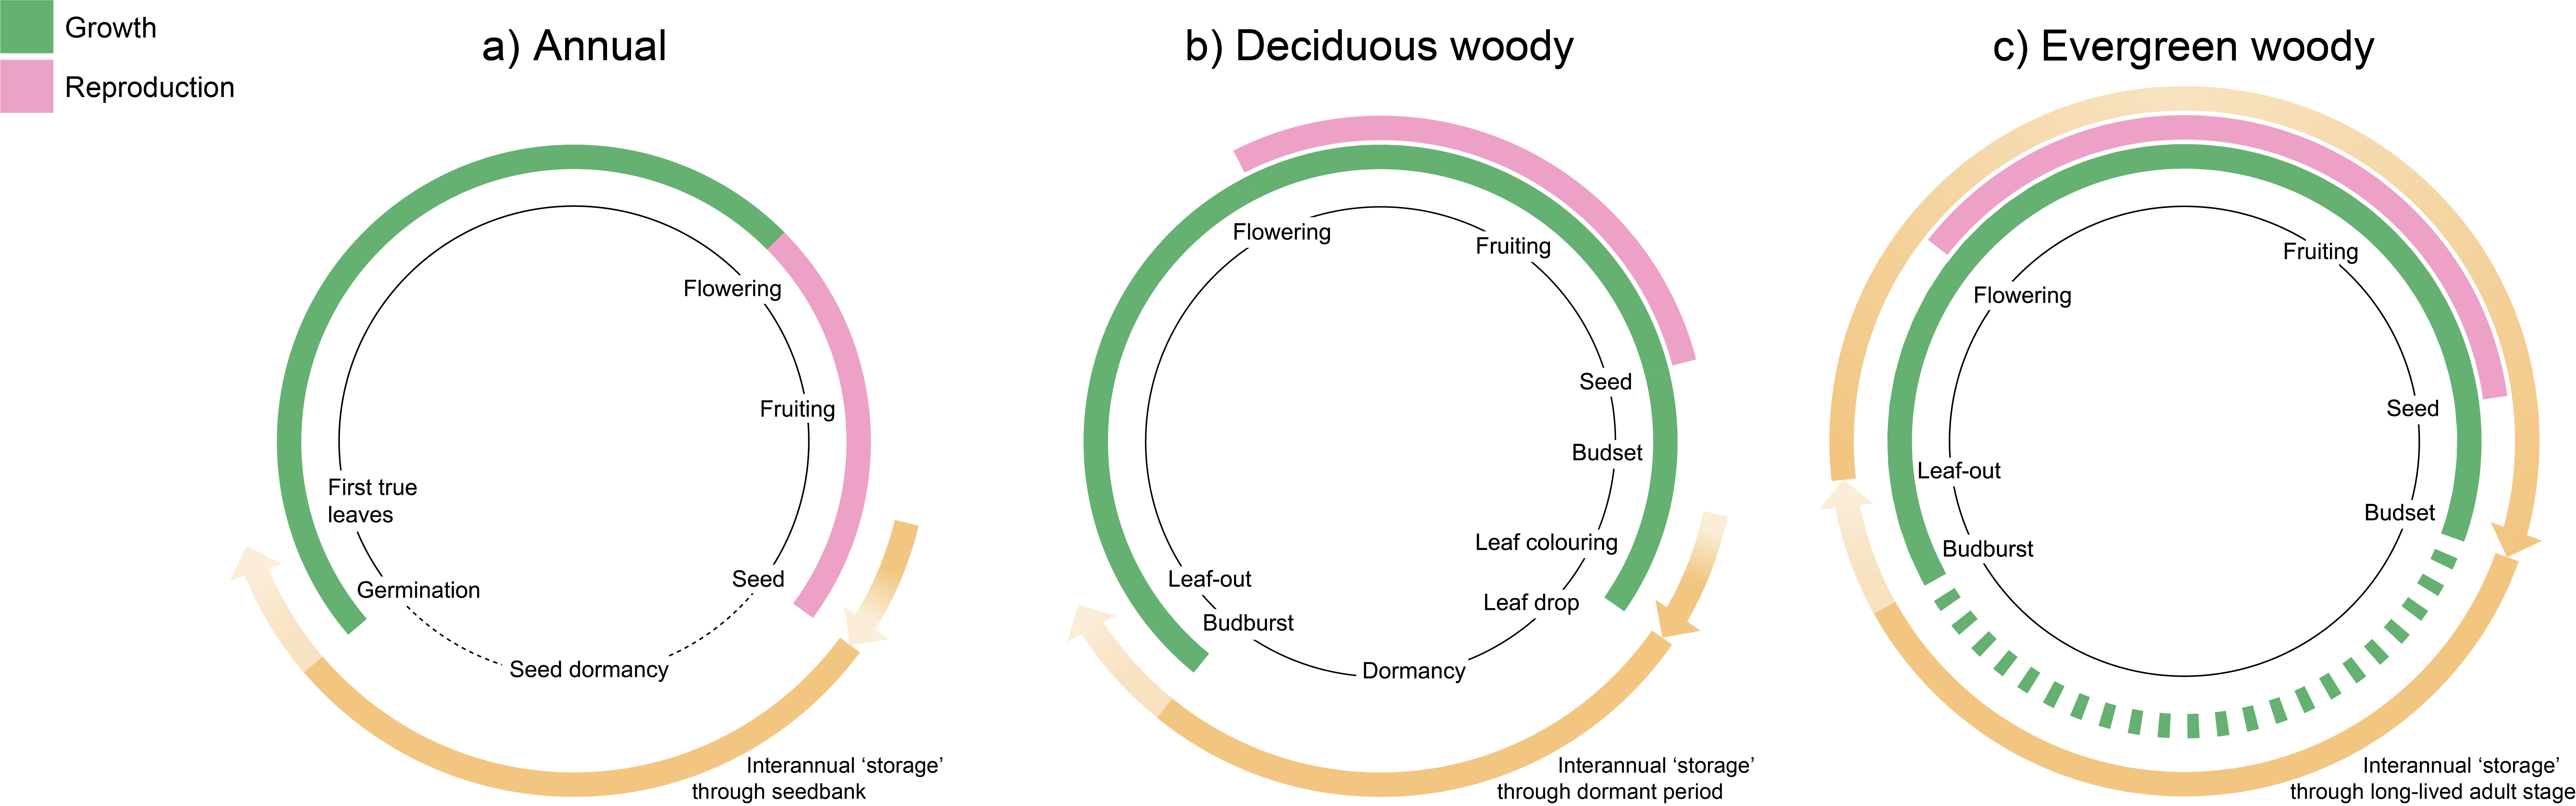
\includegraphics[width=1\textwidth]{..//figures/figsubmit/phenologyCirclesStorage.png}
\caption{Phenology captures the timing of critical stages of growth and reproduction and the transitions between them, a definition that highlights how phenology is not limited to recurring events (i.e., events that occur more than once in a lifespan) and thus spans annual (a) to perennial (b-c) life history strategies.  Plants should optimize their phenology given constraints (e.g. unfavorable climate, herbivory, necessary developmental sequences) over their lifespans in many ways that in turn impact community assembly. For example, the `storage effect' model focuses on the conceptual idea that species may demographically  `store' survivorship during environmentally favorable periods to persist through unfavorable environmental periods, and can promote coexistence of phenotypically similar species given that favorable periods also correspond to high intraspecific competition \citep[][and see text for more details]{Chesson:2000vd}. We show three examples of this `storage' here: (a) annual plants, which generally must always invest in growth first and reproduction at the end of their life, and thus store good years through their seedbanks; (b) woody deciduous species, which can generally flower and fruit at various times, but store good years through winter dormancy, and (c) evergreen woody species, which can grow throughout the year, and store through long-lived lifestages. We show reproduction mid-season for the woody species, though it can occur before leafout or much later in the season. While we show one annual cycle here, these mechanisms of `storage' often occur interannually (where unfavorable periods are some years but not others), but can also occur within a growing season. Additionally, while we do not show seedbanks for woody species, they also have them---thus having multiple ways for the storage effect to act.}
 \label{fig:phenologycircles}
\end{figure}

\clearpage


\begin{figure}[h!]
\centering
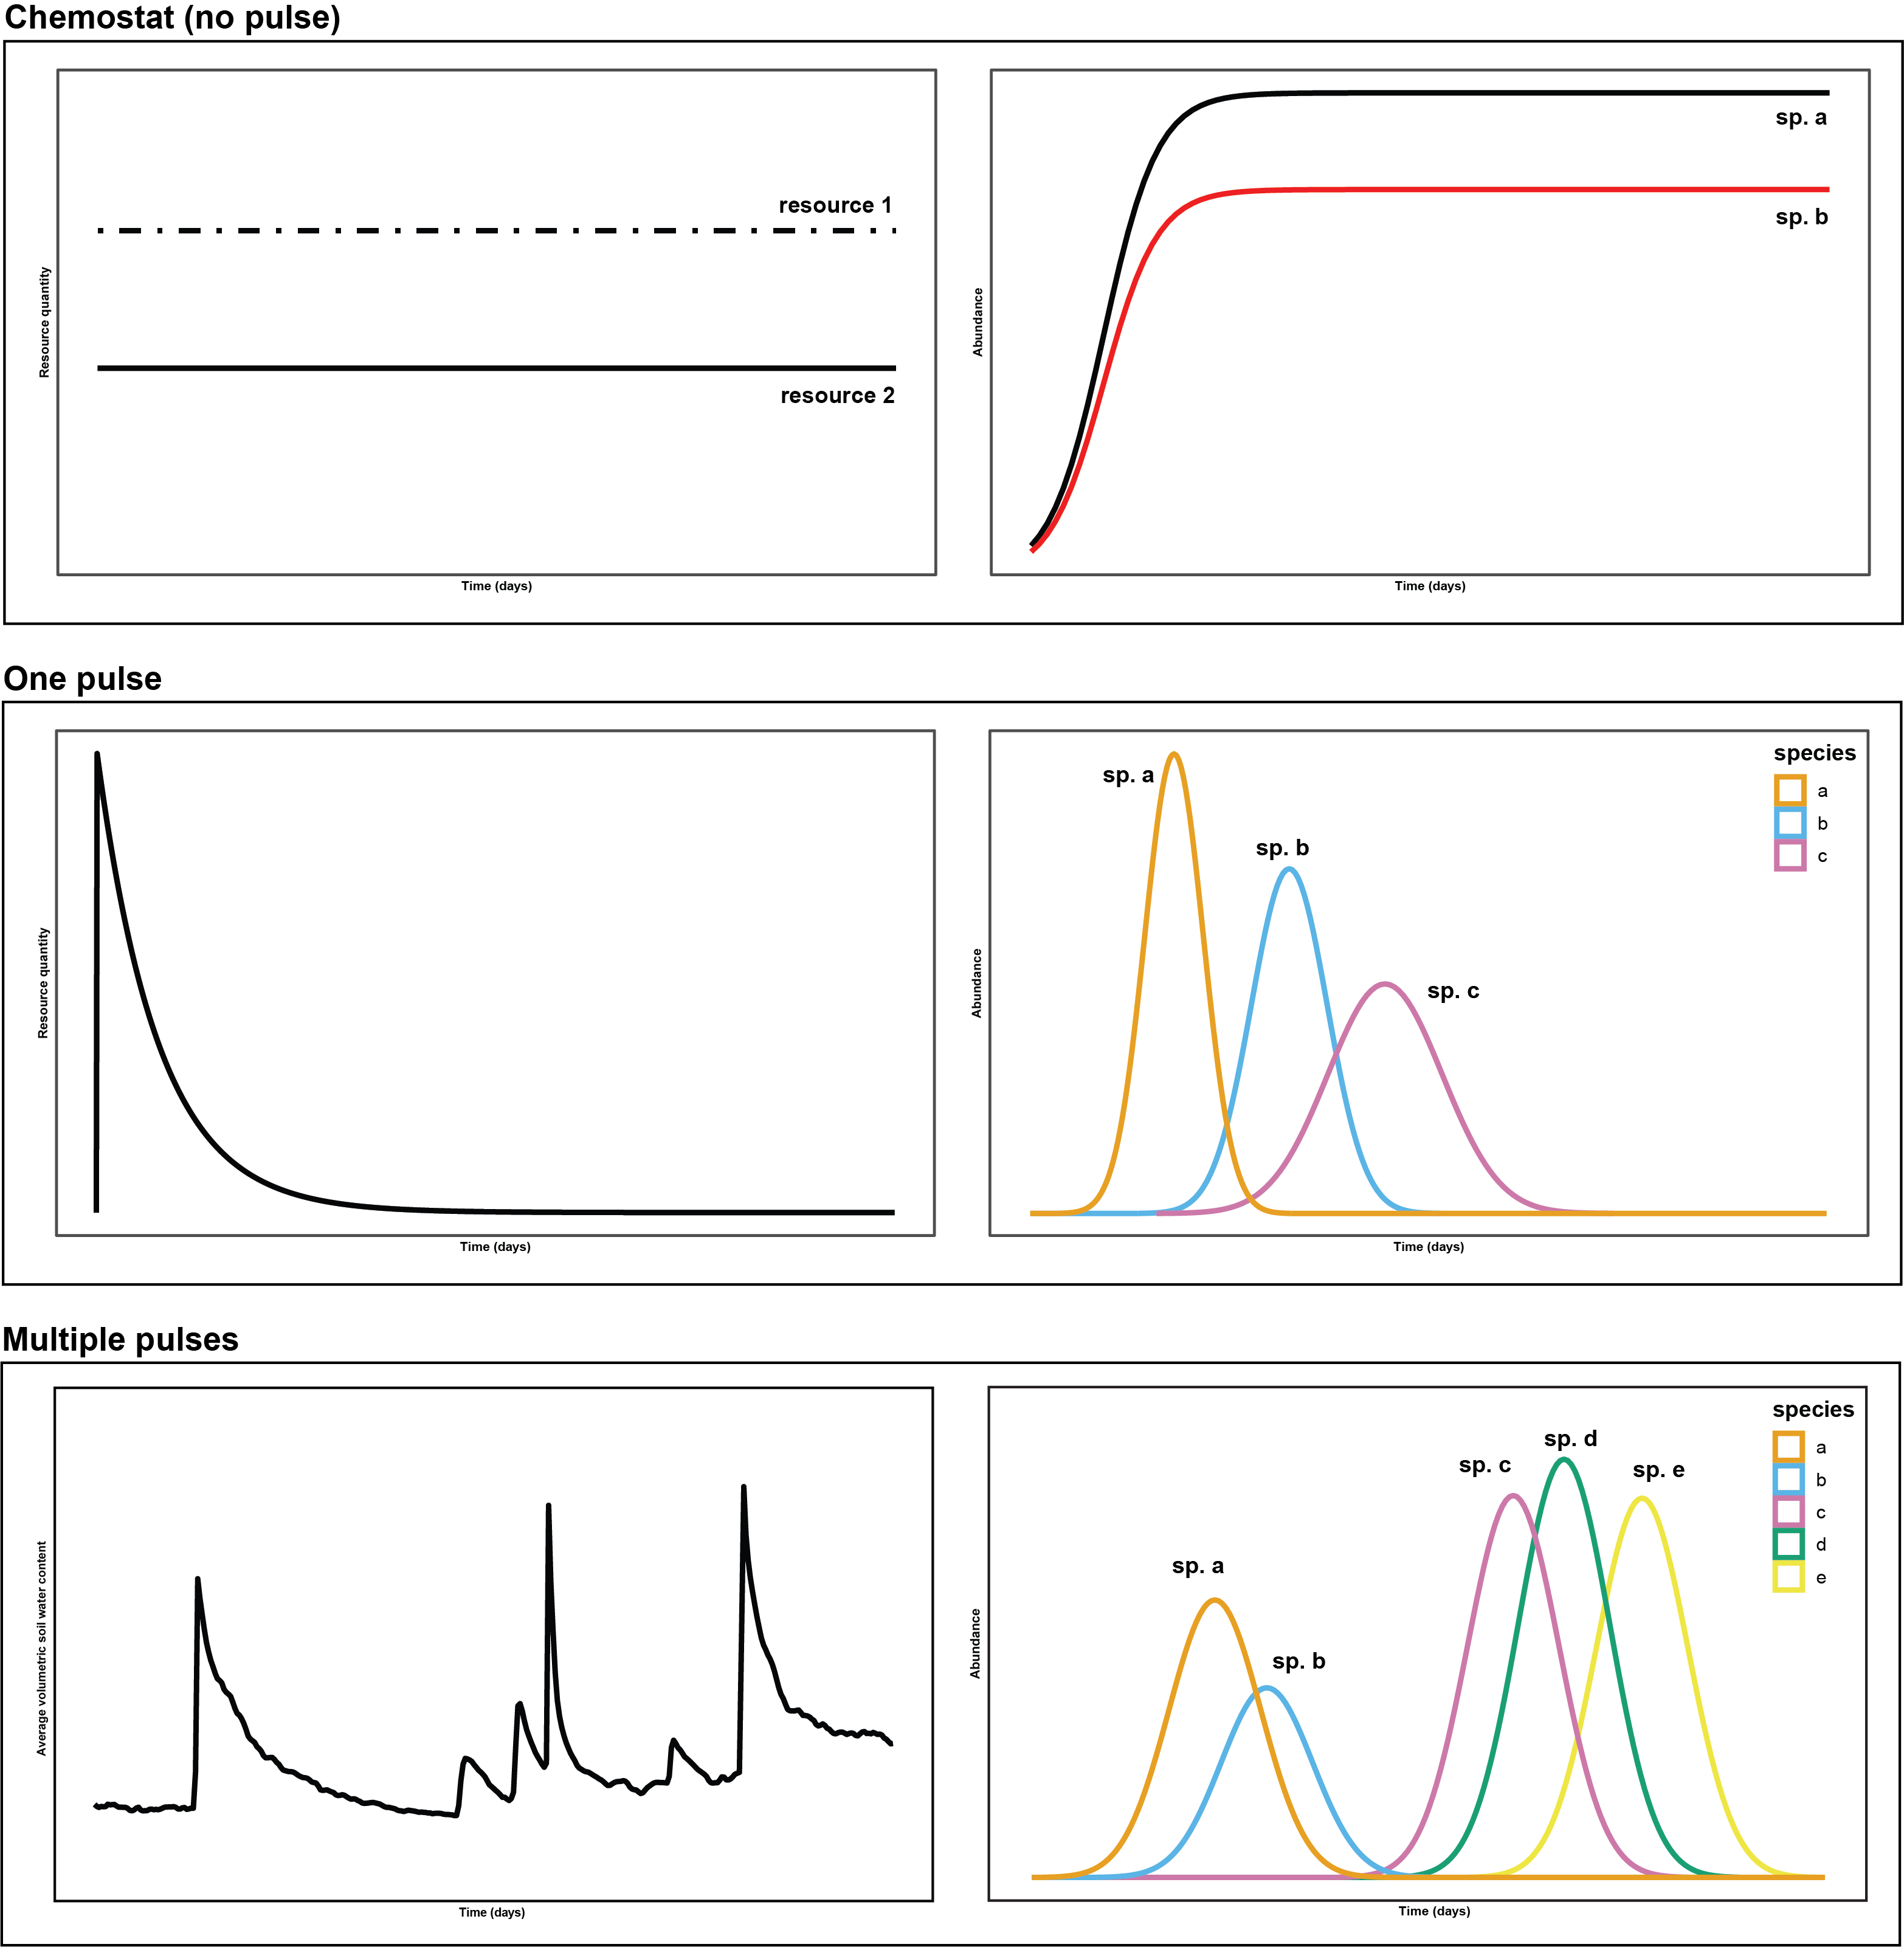
\includegraphics[width=0.8\textwidth]{..//figures/figsubmit/sixpanel_concept_increasespp.png}
\caption{Theory suggests resource levels may determine temporal niche space. In a system where resources are constant (top left, chemostat; species can only coexist if they are each the superior competitor for a different limiting resource) species would be expected to show little temporal fluctuations and there would be no real temporal niches. Many models of coexistence today, however, assume a resource pulse that decays over time (middle, left; e.g., water with evaporative loss, such as in snowpack systems): this resource then sets the temporal window of each season and species compete within it. Most real systems, however, are more complicated; multiple resource pulses could provide opportunities to partition niches temporally further: here we show hypothetical species temporal niches (bottom right) based on real soil moisture data \citep[bottom left, taken from Jornada LTER site 302, showing soil moisture at 10 cm depth over the year in 2018,][]{jornadadat}.} 

 \label{fig:resource}
\end{figure}


\begin{figure}[h!]
\centering
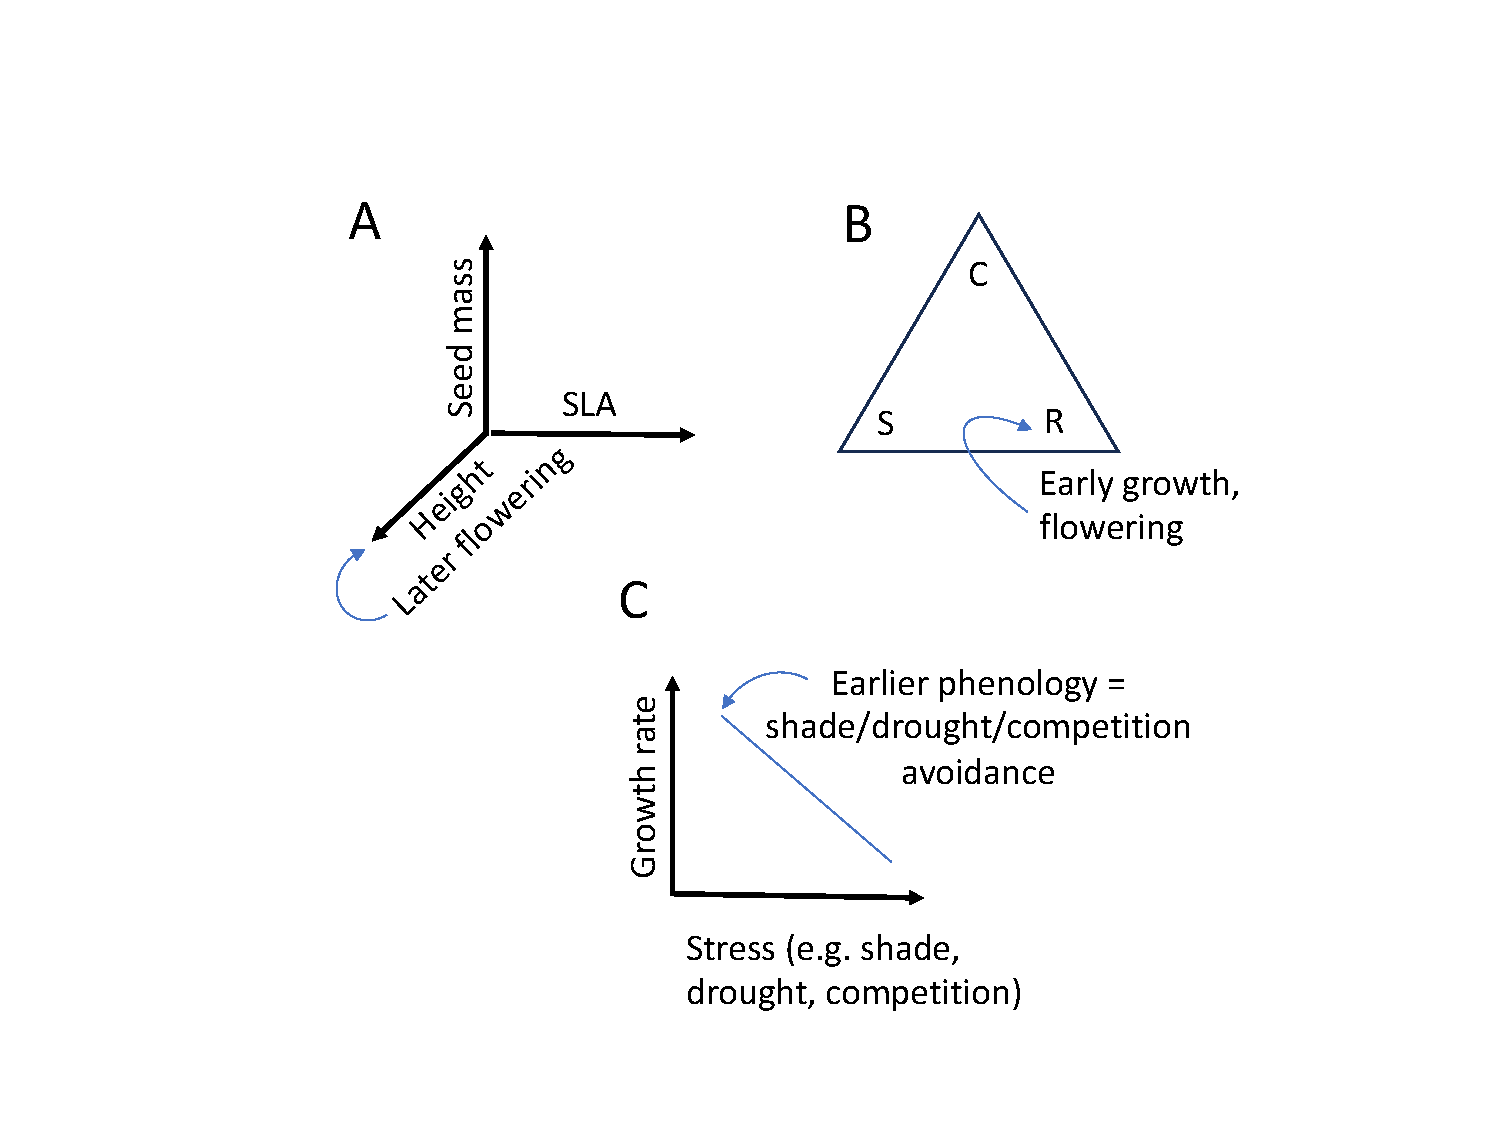
\includegraphics[width=1\textwidth]{..//figures/figsubmit/AREESfigure.pdf}
\caption{Phenology links to ecological strategies and trade-offs. For instance, in the Leaf-Height-Seed (LHS) schema greater plant height has been linked to later flowering (A). In the competitive, stress-tolerant or ruderal (CSR) plant strategy framework, earlier flowering is often observed in ruderal species (B). Earlier flowering is also associated with drought escape, shade avoidance, and escape from competition later in the growing season (C). See main text for references.}
 \label{fig:traitcorr}
\end{figure}


\begin{figure}[h!]
\centering
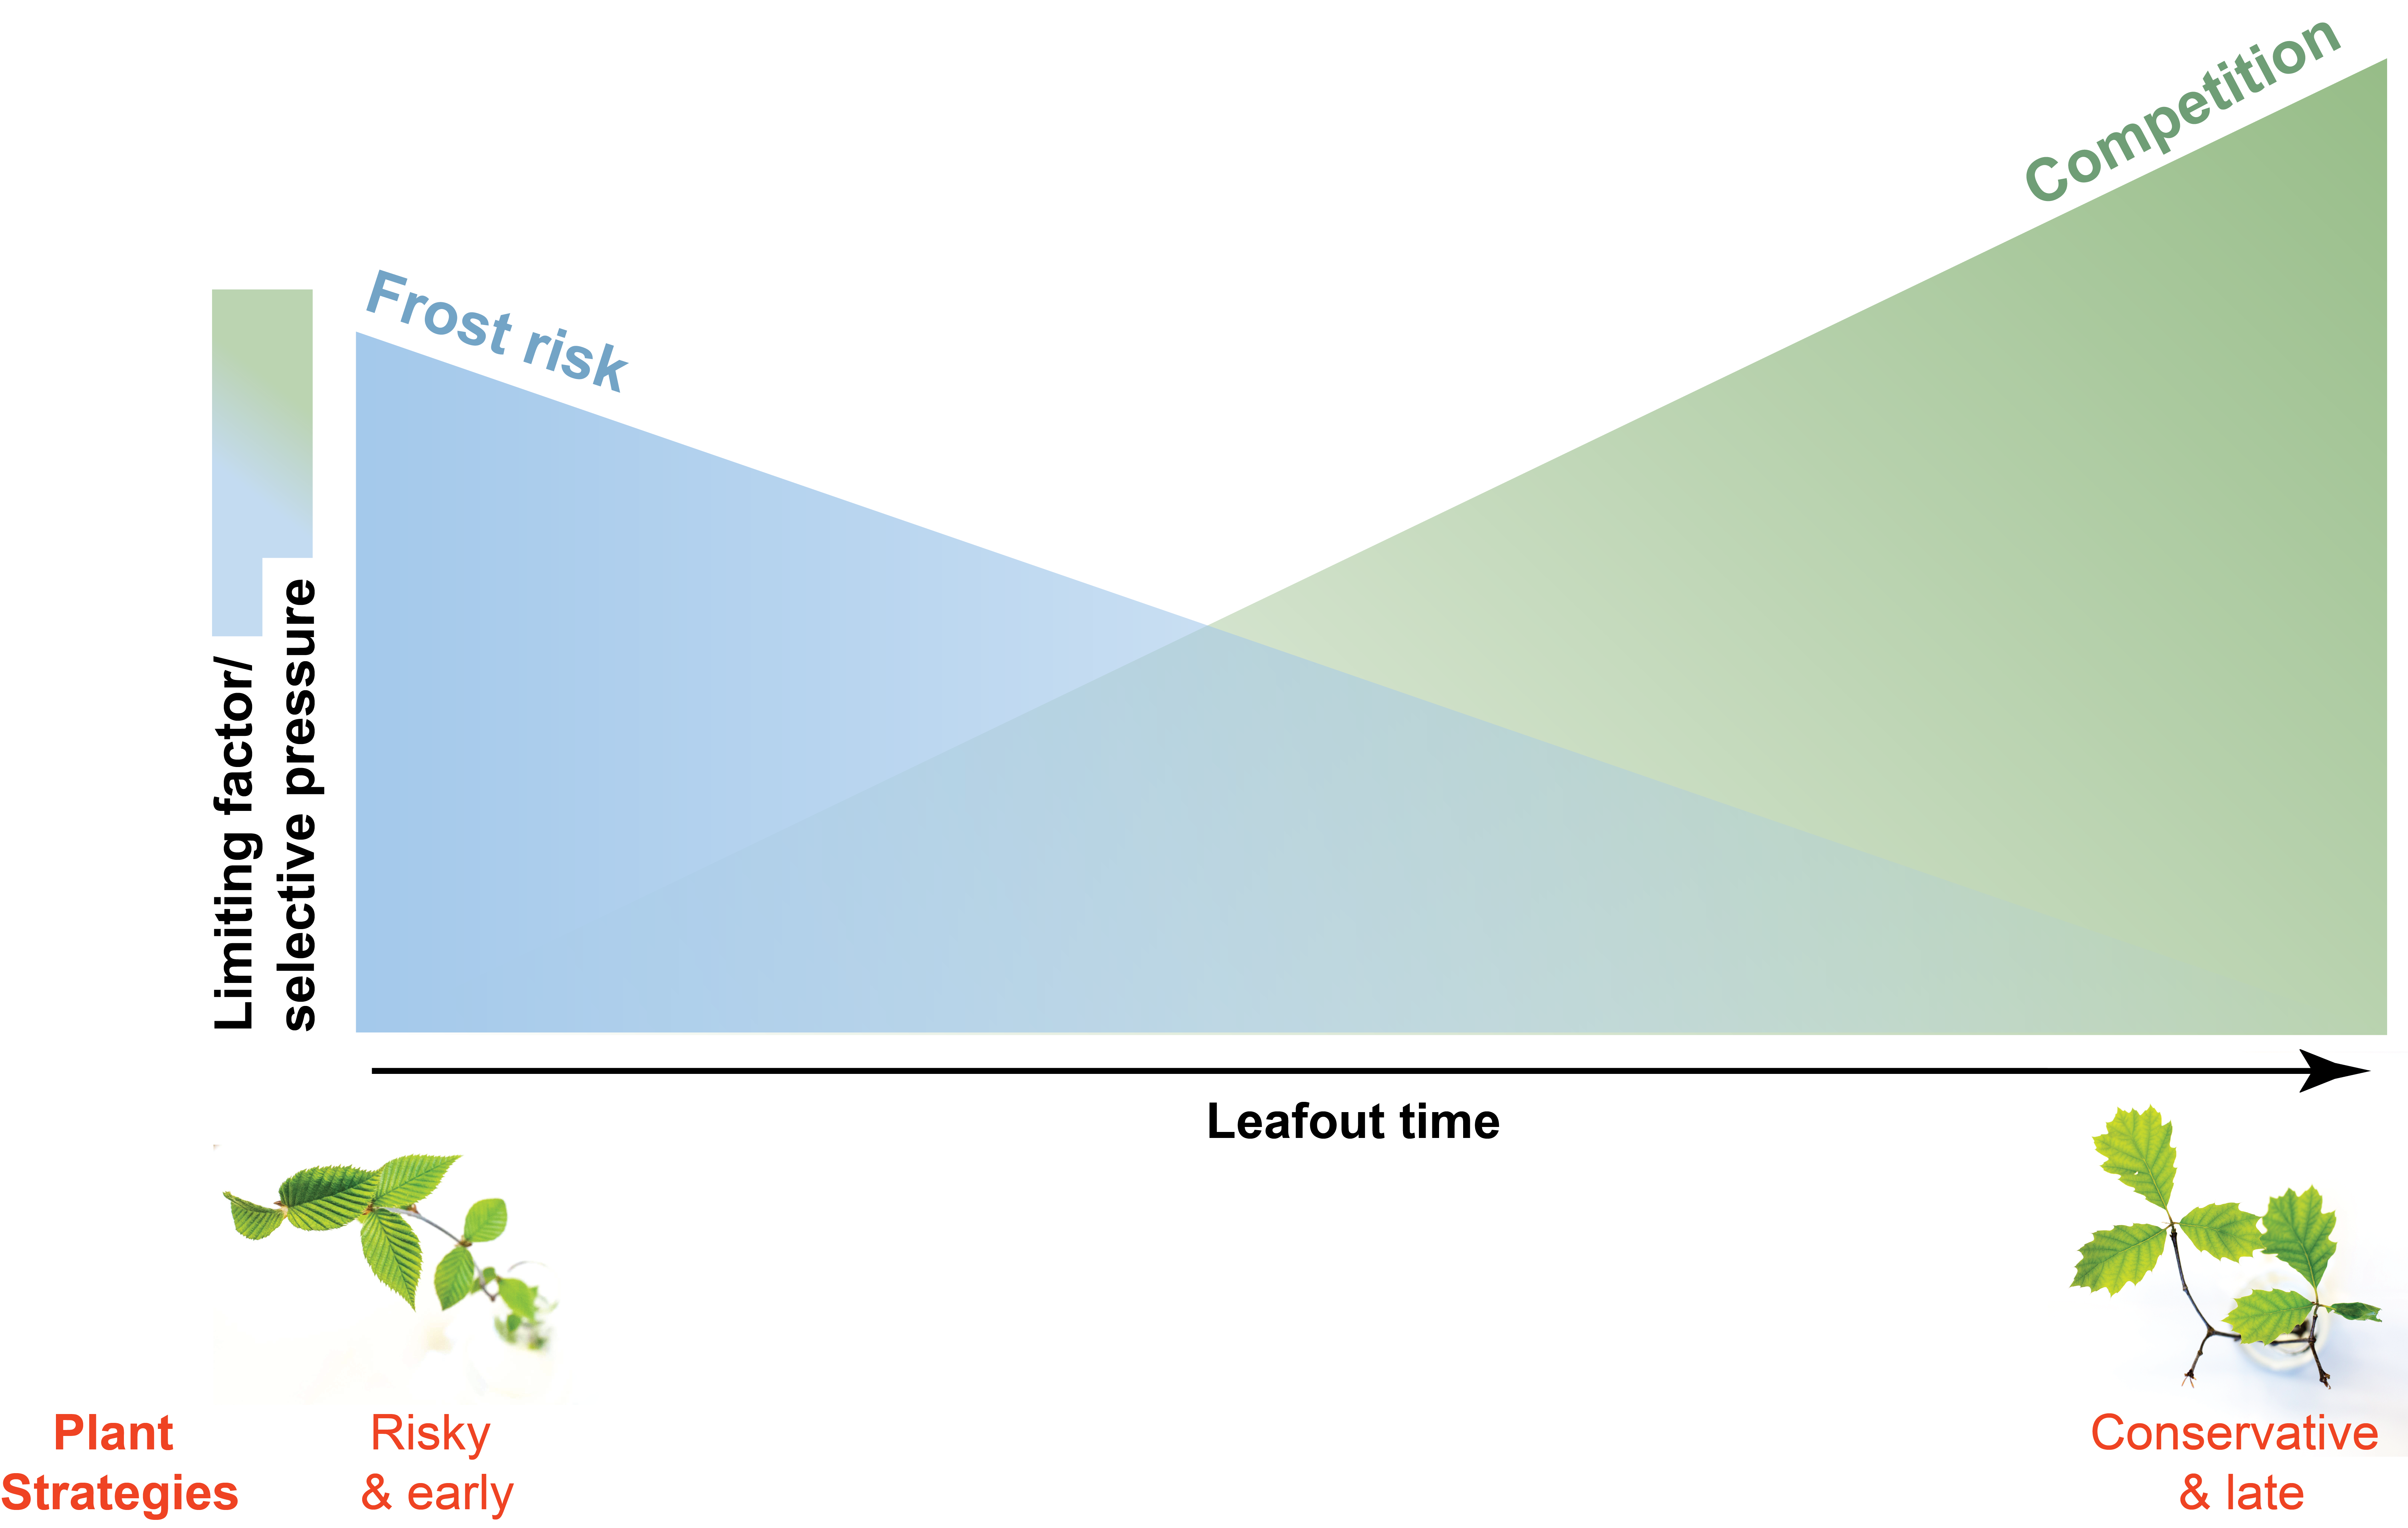
\includegraphics[width=0.9\textwidth]{..//figures/figsubmit/frosttradeoffs2.png}
\caption{In temperature systems where low temperatures generally define unfavorable periods, species may trade-off along an axis of frost risk versus a competitive environment. Early-active species (e.g., many \emph{Betula} species) risk losing tissue to frost, but gain access to more available light and soil resources while later active species  (e.g. some \emph{Quercus} species) experience almost no risk of frost but leafout and start resource uptake when many other species are active and thus competition is high. Photos by T. Savas.}
 \label{fig:seasonaltradeoffs}
\end{figure}


\end{document}

